% Chapter 3:

\chapter{High-Level Programming for Multi-GPU Systems}

\label{chapter:skelcl}

In this chapter we address the first main challenge identified in \autoref{chapter:background}: \emph{Programmability} of modern parallel systems.
We will see how structured parallel programming significantly simplifies the task of programming for parallel systems.
As throughout the thesis, we will focus on programming of single- and multi-\GPU systems.
But many observations made here are also valid when programming other parallel systems.

We will first motivate the need for high-level abstractions using a real-world \OpenCL application from the field of medical imaging.
Then we introduce the \emph{\SkelCL} programming model and its implementation as a \Cpp library which addresses the lack of high-level abstractions in state-of-the-art \GPU programming models.
The following \autoref{chapter:skelcl-evaluation} will provide several application studies to thoroughly evaluate the usefulness and performance of the abstractions and implementation presented in this chapter.


% ============================================================================ %
% ============================================================================ %
\section{The need for high-level abstractions}
We start the discussion of programming for parallel systems and in particular for \GPU systems by locking thoroughly at an application example.
By doing so we will identify challenges opposed upon application developers which arise from the parallel hardware architecture.
We will then derive from these challenges requirements to a potential high-level programming model.


% ============================================================================ %
\subsection{Challenges of \GPU programming}
\label{section:opencl-example}
We choose to investigate a real-world application rather than a simple benchmark to identify not only fundamental challenges every application developer targeting \GPU systems faces, but also practical programming challenges which become only visible for more complex applications, \eg, managing the execution of multiple compute kernels.

Our example application is the LM OSEM algorithm~\cite{ReaderErFlOt1998, SchellmannGoMeKoScWuBu2009} for image reconstruction used in Positron Emission Tomography (PET).
In PET, a radioactive substance is injected into a human or animal body, which is then placed inside a PET scanner that contains several arrays of detectors.
As the particles of the applied substance decay, positrons are emitted (hence the name PET) and annihilate with nearby electrons, such that two photons are emitted in the opposite directions (see \autoref{fig:scanner and detector}).
These ``decay events'' are registered by two opposite detectors of the scanner which records these events.
Data collected by the PET scanner are then processed by a reconstruction algorithm to obtain a resulting image.

\begin{figure}
  \centering
  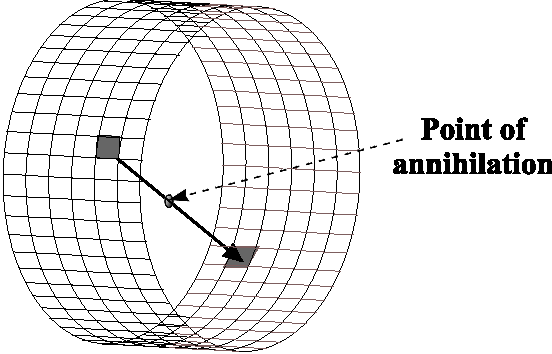
\includegraphics[scale=0.50]{ICCS/ringscanner}
  \caption{Two detectors register an event in a PET-scanner}
  \label{fig:scanner and detector}
\end{figure}

\subsubsection{The LM OSEM Algorithm}
List-Mode Ordered Subset Expectation Maximization \cite{ReaderErFlOt1998} (called LM OSEM in the sequel) is a block-iterative algorithm for 3D image reconstruction.
LM OSEM takes a set of events from a PET scanner and splits them into $s$ equally sized subsets.
Then, for each subset $S_l, l \in {0, \ldots, s-1}$, the following computation is performed:
\begin{equation}
  f_{l+1}=f_{l}c_{l};\quad c_{l}=\dfrac{1}{A_N^T \textbf{1}} \sum_{i \in S_{l}} (A_i)^T \dfrac{1}{A_{i} f_{l}}.
\label{equ:lm_osem}
\end{equation}

Here $f \in \mathbb{R}^n$ is a 3D image in vector form with dimensions $n = (X \times Y \times Z)$, $A$ it the so called system matrix, element $a_{ik}$ of row $A_i$ is the length of intersection of the line between the two detectors of event $i$ with voxel $k$ of the reconstruction image, computed with Siddon's algorithm \cite{Siddon1985}.
$\rfrac{1}{A_N^T \textbf{1}}$ is the so-called normalization vector; since it can be precomputed, we will omit it in the following.
The multiplication $f_{l}c_{l}$ is performed element-wise.
Each subset's computation takes its predecessor's output image as input and produces a new, more precise image.

The structure of a sequential LM OSEM implementation is shown in \autoref{lst:lmosem:seq_code}.
The outermost loop iterates over the subsets.
The first inner loop (step 1, lines~\autoref{lst:lmosem:seq_code:step1:begin}--\autoref{lst:lmosem:seq_code:step1:end}) iterates over subset's events to compute $c_l$, which requires three sub-steps:
row $A_i$ is computed from the current event using Siddon's algorithm;
the local error for row $A_i$ is computed and, finally, added to $c_l$.
The second inner loop (step 2, lines~\autoref{lst:lmosem:seq_code:step2:begin}--\autoref{lst:lmosem:seq_code:step2:end}) iterates over all elements of $f_l$ and $c_l$ to compute $f_{l+1}$.
\begin{figure}
\begin{lstlisting}[
  caption={Sequential code for LM OSEM comprises one outer loop with two nested inner loops.},
  label={lst:lmosem:seq_code}]
for (int l = 0; l < subsets; l++) {
  // read subset

  // step 1: compute error image $c_l$
  for (int i = 0; i < subset_size; i++) { $\label{lst:lmosem:seq_code:step1:begin}$
    // compute $A_i$
    // compute local error
    // add local error to $c_l$
  } $\label{lst:lmosem:seq_code:step1:end}$

  // step 2: update image estimate $f$
  for (int k = 0 ; k < image_size; k++) { $\label{lst:lmosem:seq_code:step2:begin}$
    if (c_l[k] > 0.0) { f[k] = f[k] * c_l[k]; }
  } $\label{lst:lmosem:seq_code:step2:end}$
}
\end{lstlisting}
\end{figure}

\subsubsection{Parallelization of LM OSEM in OpenCL}
\label{sec:parallel_implementation}
LM OSEM is a rather time-consuming algorithm that needs parallelization:
a typical 3D image reconstruction processing $6 \cdot 10^7$ input events for a $150 \times 150 \times 280$ voxel PET image takes more than two hours on a modern PC.

Although the iterations of the outer loop in \autoref{lst:lmosem:seq_code} are inherently sequential, we can parallelize the two calculation steps within one iteration as shown in \autoref{fig:lmosem:em_distribution} for a system comprising one CPU and two GPUs.
Note that these steps require different data distribution patterns:
\begin{itemize}
  \item[] \emph{Step 1:} Subset's events are copied from the CPU to all GPUs (\emph{upload}) to compute the summation part of $c_l$ concurrently. This step requires that the complete image estimate $f_l$ is available to all GPUs.
  \item[] \emph{Step 2:} For computing the next image estimate $f_{l+1}$ in parallel, the current image estimate $f_l$ and the error image $c_l$ computed in step 1 have to be distributed in disjoint parts (blocks) among all GPUs.
\end{itemize}

\begin{figure}
  \centering
  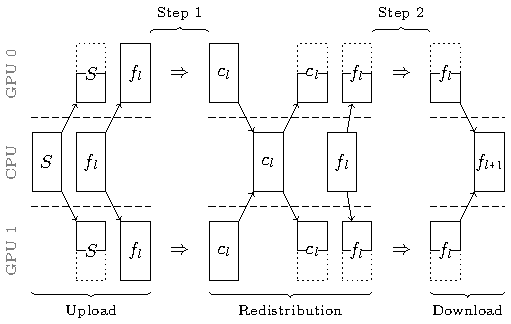
\includegraphics[width=0.6\textwidth]{ICCS/em_distribution}
  \caption{Parallelization schema of the LM OSEM algorithm.}
  \label{fig:lmosem:em_distribution}
\end{figure}
Thus, the parallelization schema in \autoref{fig:lmosem:em_distribution} requires a data \emph{redistribution} phase between the two computation steps.
During step 1, each GPU computes a partial sum of $c_l$ which are summed up and redistributed disjoinlty to all GPUs after step 1.
Note that for step 1, each GPU requires a full copy of the image estimate, while in step 2 all GPUs update disjoint parts of it.
After step 2, the disjoint parts of the image estimate are copied from all GPUs back to the CPU (\emph{download}).

\bigskip\noindent
In the following, we describe how the phases in the parallelization schema in \autoref{fig:lmosem:em_distribution} are implemented using OpenCL.

\paragraph{Upload}
\autoref{lst:lmosem:upload} shows the simplified OpenCL implementation of the upload phase.
Uploading of the event vector $S$ is performed in lines \autoref{lst:lmosem:upload:1:start}--\autoref{lst:lmosem:upload:1:end}, while lines \autoref{lst:lmosem:upload:2:start}--\autoref{lst:lmosem:upload:2:end} show the upload of the image estimate $f_l$.
In OpenCL, we have to manage each GPU explicitly, therefore, for each GPU, we create an array of buffers (\texttt{s\_gpu} in line~\autoref{lst:lmosem:upload:1:cl_false} and \texttt{f\_gpu} in line~\autoref{lst:lmosem:upload:2:cl_false}) and we use a loop (line \autoref{lst:lmosem:upload:loop}) to repeat all memory operations for each GPU.
For performance reasons, we use asynchronous copy operations, specified using the \texttt{CL\_FALSE} flag (lines \autoref{lst:lmosem:upload:1:cl_false} and \autoref{lst:lmosem:upload:2:cl_false}): this allows data transfers to multiple GPUs to overlap.
We perform different operations with $S$ (distribute among all GPUs) and $f_l$ (copy to each GPU), therefore, there are differences when specifying the amount of bytes to copy (lines \autoref{lst:lmosem:upload:1:amount} and \autoref{lst:lmosem:upload:2:amount}) and the offsets in the CPU memory (lines \autoref{lst:lmosem:upload:1:offset} and \autoref{lst:lmosem:upload:2:offset}).
Altogether eleven such memory operations -- each with different amounts of bytes and offsets -- appear in the OpenCL source code.

\begin{lstlisting}[float,
  caption={Implementation of the upload phase in OpenCL (omitting error checks for brevity)},
  label={lst:lmosem:upload}]
for (int gpu = 0; gpu < gpu_count; gpu++) {$\label{lst:lmosem:upload:loop}$
  // upload $S$
  clEnqueueWriteBuffer( command_queue[gpu], $\label{lst:lmosem:upload:1:start}$
        s_gpu[gpu], CL_FALSE, 0,$\label{lst:lmosem:upload:1:cl_false}$
        sizeof(float) * size_of_s / gpu_count,$\label{lst:lmosem:upload:1:amount}$
        (void*)&s_cpu[ gpu * size_of_s / gpu_count ],$\label{lst:lmosem:upload:1:offset}$
        0, NULL, NULL );$\label{lst:lmosem:upload:1:end}$

  // upload $f_l$
  clEnqueueWriteBuffer( command_queue[gpu], $\label{lst:lmosem:upload:2:start}$
        f_gpu[gpu], CL_FALSE, 0,$\label{lst:lmosem:upload:2:cl_false}$
        sizeof(float) * size_of_f,$\label{lst:lmosem:upload:2:amount}$
        (void*)&f_cpu[0],$\label{lst:lmosem:upload:2:offset}$
        0, NULL, NULL );$\label{lst:lmosem:upload:2:end}$
}
\end{lstlisting}

\paragraph{Step 1}
The implementation of step 1 performs the operations shown in \autoref{lst:lmosem:seq_code}.
Because of GPU memory restrictions, the OpenCL implementation is not straightforward, therefore, we will not show the detailed code here.
An OpenCL kernel is launched where each work item processes multiple events one after another.
For each event first $A_i$ is computed, then the local error for $A_i$ computed using the current image estimate $f_l$ which is finally added to $c_l$.

In the formula $A_i$ represents the \emph{path} of a detected line through the 3D image space.
In mathematics it is convenient to think as this as a sparse vector containing the length of the intersection of the line with a given voxel in the image space.
As most voxels are not intersected by the line, most entries in the vector remain zero.
Therefore, in the OpenCL code $A_i$ is represented as an array of pairs, where the first entry of each pair is the index of an voxel in the image space and the second entry is the length of the intersection with this voxel.

Synchronization between work items in OpenCL is highly restricted, \ie, synchronization is only possible for work items organized in the same work group.
Therefore, it is not possible to efficiently protect the writing operation to $c_l$ to avoid race conditions.
We have conducted studies and found that for this particular algorithm these race conditions are acceptable as they do not substantially decrease the numerical accuracy of the computed result~\cite{SchellmannGoMeKoScWuBu2009}.


\paragraph{Redistribution}

\begin{lstlisting}[float,
  caption={OpenCL pseudocode for the redistribution phase},
  label={lst:lmosem:redistribution}]
// download all c_l values from the GPUs to the CPU
cl_event events[gpu_count];
for (int gpu = 0; gpu < gpu_count; gpu++) {
  clEnqueueReadBuffer( ..., &events[gpu] );$\label{lst:lmosem:redistribution:operation}$
}
clWaitForEvents(gpu_count, events);$\label{lst:lmosem:redistribution:wait}$

// combine data on CPU
combine( ... );$\label{lst:lmosem:redistribution:combine}$

// upload block of the new c_l version to each GPU
for (int gpu = 0; gpu < gpu_count; gpu++) {
  clEnqueueWriteBuffer( ... );
}
\end{lstlisting}

\autoref{lst:lmosem:redistribution} shows an OpenCL pseudocode for the redistribution phase.
To download the data from all GPUs, we use the \texttt{clEnqueueReadBuffer} function and perform the operations asynchronously, but this time, we have to wait for the operations to finish.
For such synchronization, OpenCL uses \emph{events}, associated with an operation (line \autoref{lst:lmosem:redistribution:operation}) for waiting for the operation to finish (line \autoref{lst:lmosem:redistribution:wait}).
After all downloads have finished, we combine the different values of $c_l$ to a new value of $c_l$ on the CPU (line \autoref{lst:lmosem:redistribution:combine}), and upload the blocks of $c_l$ to the GPUs.
Even if we only copied data between GPUs, without processing them on the CPU, we still would have to download them to the CPU because direct GPU-to-GPU transfers are currently not possible in OpenCL.

\paragraph{Step 2}
\autoref{lst:lmosem:step_2} shows the implementation of step 2.
In OpenCL, computations are specified as \emph{kernels} which are created from the source code specifying the computation.
The computation in step 2 is, therefore, described as a string in lines \autoref{lst:lmosem:step_2:string:start}--\autoref{lst:lmosem:step_2:string:stop}.
The operations used here are the same as in the sequential code.

For executing the computations of step 2, we have to perform the following steps for each GPU:
\begin{itemize}
  \item create an OpenCL kernel from the source code (requires 50 lines of code in OpenCL);
  \item compile the kernel specifically for the GPU (requires 13 lines of code in OpenCL);
  \item specify kernel arguments one-by-one using the \texttt{clSetKernelArg} function (line \autoref{lst:lmosem:step_2:args:start} -- \autoref{lst:lmosem:step_2:args:stop});
  \item specify execution environment, i.\,e., how many instances of the kernel to start (line \autoref{lst:lmosem:step_2:env:start} -- \autoref{lst:lmosem:step_2:env:stop});
  \item launch the kernel (line \autoref{lst:lmosem:step_2:kernel:start} -- \autoref{lst:lmosem:step_2:kernel:stop}).
\end{itemize}
\begin{lstlisting}[float,
  caption={Implementation of step 2 in OpenCL (omitting error checks for brevity)},
  label={lst:lmosem:step_2}]
// step 2 (in $\autoref{fig:lmosem:em_distribution}$)
source_code_step_2 =
  "kernel void step2(global float* f, global float* c_l,$\label{lst:lmosem:step_2:string:start}$
                     int offset, int size) {
    int id = get_global_id(0) + offset;
    if (id < size && c_l[id] > 0.0){ f[id] = f[id]*c_l[id];}$\label{lst:lmosem:step_2:zip}$
   }";$\label{lst:lmosem:step_2:string:stop}$

for (int gpu = 0; gpu < gpu_count; gpu++) {
  // create kernel (50 lines of code)
  // compile kernel (13 lines of code)

  // specifying kernel arguments:
  clSetKernelArg(kernel_step2[gpu], 0, sizeof(cl_mem),$\label{lst:lmosem:step_2:args:start}$
                 (void*)&f_buffer[gpu]);
  clSetKernelArg(kernel_step2[gpu], 1, sizeof(cl_mem),
                 (void*)&c_l_buffer[gpu]);
  int offset = gpu * (size_of_f / gpu_count);
  clSetKernelArg(kernel_step2[gpu], 2, sizeof(int),
                 (void*)&offset);
  int size   = MIN( (gpu + 1) * (size_of_f / gpu_count),
                    size_of_f );
  clSetKernelArg(kernel_step2[gpu], 3, sizeof(int),
                 (void*)&size);$\label{lst:lmosem:step_2:args:stop}$

  // specify execution environment
  int local_work_size[1]  = { 32 };$\label{lst:lmosem:step_2:env:start}$
  int global_work_size[1] =
        { roundUp(32, size_of_f / gpu_count) };$\label{lst:lmosem:step_2:env:stop}$
  // launch the kernel
  clEnqueueNDRangeKernel($\label{lst:lmosem:step_2:kernel:start}$
        command_queue[gpu], kernel_step2[gpu],
        1, NULL, &global_work_size, &local_work_size, 0,
        NULL, NULL); }$\label{lst:lmosem:step_2:kernel:stop}$
\end{lstlisting}


\paragraph{Download}
The implementation of the download phase is similar to the upload phase as shown in \autoref{lst:lmosem:upload}.


% ============================================================================ %
\subsection{Requirements to a High-Level Programming Model}
\label{section:requirements}
The described implementation of the example application reveals the main problems and challenges that application developers have to overcome when targeting \GPU systems.
Our analysis show that to simplify programming for a system with multiple \GPUs, at least the following three high-level abstraction are desirable:

\paragraph{Parallel container data types}
Compute intensive applications typically operate on a (possibly big) set of data items.
As shown in \autoref{lst:lmosem:upload}, managing memory is error-prone because low-level details, like offset calculations, have to be programmed manually.

A high-level programming model should be able to make collections of data automatically accessible to all processors in a system and it should provide an easy-to-use interface for the application developer.

\paragraph{Recurring patterns of parallelism}
While each application (of course) performs different concrete operations, the general structure of parallelization resembles parallel patterns that are commonly used in many applications.
In step~1, for computing the error image~$c_l$, the same sequence of operations is performed for every event from the input subset, which is the well-known \emph{map} pattern of data-parallel programming~\cite{GorlatchCo2011}.
In step~2, two images (the current image estimate~$f_l$ and the error image~$c_l$) are combined element-wise into the output image~($f_{l+1}$), see line~\autoref{lst:lmosem:step_2:zip} of \autoref{lst:lmosem:step_2}, which is again a well-known pattern of parallelism commonly called \emph{zip}.

It would be, therefore, desirable to express the high-level structure of an application using pre-defined common patterns, rather than describing the parallelism manually in much detail.

\paragraph{Distribution and redistribution mechanisms}
To achieve scalability of applications on systems comprising multiple \GPUs, it is crucial to decide how the application's data are distributed across all available \GPUs.
Distributing and re-distributing data in \OpenCL is cumbersome because data transfers have to be managed manually and performed via the \CPU, as shown in \autoref{lst:lmosem:upload} and \autoref{lst:lmosem:redistribution}.

Therefore, it is important for a high-level programming model to allow both for describing the data distribution and for changing the distribution at runtime.


% ============================================================================ %
% ============================================================================ %
\section{The SkelCL Programming Model}
\label{section:skelcl-programming-model}
\SkelCL (Skeleton Computing Language) is a high-level programming model targeting multi-\GPU system.
It is developed as an extension of the standard \OpenCL programming model~\cite{OpenCL}.

\SkelCL adds three main high-level features to \OpenCL which we identified as desirable in~\autoref{section:requirements}:

\begin{itemize}
  \item \emph{parallel container data types} for unified memory management between \CPU and (multiple) \GPUs;
  \item \emph{recurring patterns of parallelism} (\aka \emph{algorithmic skeletons}) for easily expressing parallel computation patterns;
  \item \emph{data distribution} and \emph{redistribution} mechanisms for transparent data transfers in multi-\GPU systems.
\end{itemize}

\noindent
\SkelCL inherits all advantageous properties of \OpenCL, including its portability across different heterogeneous parallel systems.
\SkelCL is designed to be fully compatible with \OpenCL: arbitrary parts of a \SkelCL code can be written or rewritten in \OpenCL, without influencing program's correctness.

In the remainder of this section we discuss the design of the \SkelCL programming model in more detail.
Its implementation as a \Cpp library will be discussed in the next section.

% ============================================================================ %
\subsection{Parallel Container Data Types}
\label{section:skelcl-programming-model:container}
\SkelCL offers the application developer two container classes -- vector and matrix -- which are transparently accessible by both, \CPU and \GPUs (or using \OpenCL's terminology, host and devices).
The \emph{vector} abstracts a one-dimensional contiguous memory area while the \emph{matrix} provides an interface to a two-dimensional memory area.
The \SkelCL container data types have two major advantages as compared with \OpenCL.

The first advantage is its automatic memory management.
When a container is created on the host, memory is allocated on the devices automatically;
when a container on the host is deleted, the memory allocated on the devices is freed automatically.
In \OpenCL memory has to be allocated and freed manually.

The second advantage is that the necessary data transfers between the host and devices are performed automatically and implicitly.
Before performing a computation on container types, the \SkelCL system ensures that all input containers' data is available on all participating devices.
This may result in implicit data transfers from the host to device memory, which in \OpenCL requires explicit programming, as we saw in~\autoref{lst:lmosem:upload} in~\autoref{section:opencl-example}.
Similarly, before any data is accessed on the host, the implementation of \SkelCL implicitly ensures that this data on the host is up-to-date by performing necessary data transfers automatically.
Using the \code{clEnqueueWriteBuffer} (see lines~\ref{lst:lmosem:upload:1:start}--\ref{lst:lmosem:upload:1:end} in \autoref{lst:lmosem:upload}) and \code{clEnqueueReadBuffer} (see \autoref{lst:lmosem:redistribution}) functions nine arguments have to be specified to perform a single data transfer in \OpenCL.
The \SkelCL container classes shield the programmer from these low-level operations like memory allocation (on the devices) and data transfers between host and device.

Developing applications on two-dimensional data for modern parallel architectures is cumbersome and challenging, since efficient memory handling is essential for achieving good performance.
In case of \GPUs, exploiting the memory hierarchy by using the fast but small on-chip memory is key for high performance.
Therefore, in addition to the vector as a one-dimensional abstract data structure, \SkelCL offers a specific abstract data type for handling two-dimensional data, the matrix.
We will see later in \autoref{sec:opt_allpairs_skeleton} and \autoref{section:skelcl-library} how \SkelCL automatically exploits the memory hierarchy to improve performance.

% The implementations of the algorithmic skeletons included in \SkelCL differentiate for their input container between vector and matrix, thus, offering optimized implementations for each case.


\subsection{Algorithmic Skeletons}
\label{section:skelcl-programming-model:skeletons}
In original \OpenCL, computations are expressed as compute \emph{kernels} which are executed in a parallel manner on an \OpenCL device, \eg, a \GPU.
As seen earlier in \autoref{section:opencl-example} the application developer must explicitly specify the parallelism by indicating how many instances of a kernel (called \emph{work items}) should be launched in parallel.
In \autoref{lst:lmosem:step_2} the \code{local\_work\_size} (line~\ref{lst:lmosem:step_2:env:start}) and \code{global\_work\_size} (line~\ref{lst:lmosem:step_2:env:global}) specify the number of work items and how they are organized into groups.
The programmer must ensure that these numbers match,\ie, that the global size is evenly divisible by the local size.
Communications between work items are limited and have to be implemented carefully to avoid race conditions and deadlocks.
In addition, kernels take pointers to device memory as input and contain program code for reading/writing single data items from/to it.
These pointers are unsafe as they have to be used carefully, because no boundary checks are performed by \OpenCL.

To shield the application developer from these low-level programming issues, \SkelCL extends \OpenCL by introducing high-level programming patterns, called \emph{algorithmic skeletons}~\cite{Cole1991}.
Formally, a skeleton is a higher-order function that executes one or more user-defined (so-called \emph{customizing}) functions in a pre-defined parallel manner, thus hiding the details of parallelism and communication from the user~\cite{GorlatchCo2011}.

\SkelCL provides four basic data-parallel skeletons: \map, \zip, \reduce, and \scan,
as well as two more advanced skeletons targeting specific application domains: \stencil and \allpairs.
In this section we will look at the basic skeletons, the advanced skeletons will be discussed in~\autoref{section:skelcl-programming-model:specialSkeletons}.
The four basic skeletons have been selected, because they have been proven to be useful for a broad range of applications.
Moreover, these skeletons can be efficiently implemented on \GPUs as their computation patterns match the data-parallel \SIMD (Singe Instruction, Multiple Data) execution model implemented by \GPUs.


\paragraph{The \map skeleton}
The \map skeleton is a well-known basic algorithmic skeleton, applying the customizing function to each element of a container in parallel.
This skeleton originates from the functional world, where the \code{map} function is recognized as an important primitive for writing high-level code.
In many programming languages an equivalent sequential function exists, either known under the same name, like in Haskell or Python, or by other names, like \code{transform} in \Cpp.

In \SkelCL the \map skeleton can operate on vectors as well as matrices.
We start by formally defining the skeleton on vectors:
\begin{definition}
  \label{definition:map}
  Let $\vec{x}$ be a vector of size $n$ with elements $x_i$ where $0 < i \leq n$.
  Let $f$ be a unary customizing function defined on elements.
  The algorithmic skeleton \map is then defined as follows:
  \begin{equation*}
    \map\ f\ [x_1, x_2, \dots, x_n] \eqdef [f\ x_1, f\ x_2, \dots, f\ x_n]
  \end{equation*}
\end{definition}
\noindent
The definition for matrices is similar:
\begin{definition}
  \label{definition:map:matrix}
  Let $M$ be an $n\times m$ matrix with elements $m_{i,j}$ where $0 < i \leq n$ and $0 < j \leq m$.
  Let $f$ be a unary customizing function.
  The algorithmic skeleton \map is defined as follows:
  \begin{equation*}
    \map\ f\ \DottedMatrix{m_{0,0}}{m_{0,m}}{m_{n,0}}{m_{n,m}}
      \eqdef \DottedMatrix{f\ m_{0,0}}{f\ m_{0,m}}{f\ m_{n,0}}{f\ m_{n,m}}
  \end{equation*}
\end{definition}
\noindent
The output container of the \map skeleton, either vector or matrix, can be computed in parallel, because the computation of each single element is independent of each other.

A simple possible application of the \map skeleton is negating all the values in a vector:
\begin{align*}
  neg\ \vec{x} &= \map\ (-)\ \vec{x}
\end{align*}


\paragraph{The \zip skeleton}
The \zip skeleton operates on two containers and combines them into one.
As the \map skeleton it is defined for vectors and matrices as well.
\begin{definition}
  \label{definition:zip}
  Let $\vec{x}$ and $\vec{y}$ be vectors of size $n$ with elements $x_i$ and $y_i$ where $0 < i \leq n$.
  Let $\oplus$ be a binary customizing operator.
  The algorithmic skeleton \zip is defined as follows:
  \begin{equation*}
    \begin{split}
      \zip\ \oplus\ [x_1, x_2, \dots, x_n]\ [y_1, y_2, \dots, y_n]\\
      \eqdef [x_1 \oplus y_1, x_2 \oplus y_2, \dots, x_n \oplus y_n]
    \end{split}
  \end{equation*}
\end{definition}
\noindent
Again the definition for matrices is similar:
\begin{definition}
  \label{definition:zip:matrix}
  Let $M$ and $N$ be $n\times m$ matrices with elements $m_{i,j}$ and $n_{i,j}$ where $0 < i \leq n$ and $0 < j \leq m$.
  Let $\oplus$ be a binary customizing operator.
  The algorithmic skeleton \zip is defined as follows:
  \begin{equation*}
    \begin{split}
      \zip\ f\ {\DottedMatrix{m_{0,0}}{m_{0,m}}{m_{n,0}}{m_{n,m}}}\
            {\DottedMatrix{n_{0,0}}{n_{0,m}}{n_{n,0}}{n_{n,m}}} \\
      \eqdef \DottedMatrix{m_{0,0} \oplus n_{0,0}}{m_{0,m} \oplus n_{0,m}}{m_{n,0} \oplus n_{n,0}}{m_{n,m} \oplus n_{n,m}}
    \end{split}
  \end{equation*}
\end{definition}
\noindent
This definitions require the two input containers to be of exactly the same size.
The \zip skeleton is parallelizeable in the same manner as \map, as each element of the output container can be computed in parallel.

A possible application of the \zip skeleton is performing pairwise addition of two vectors:
\begin{align*}
  add\ \vec{x}\ \vec{y} = \zip\ (+)\ \vec{x}\ \vec{y}
\end{align*}


\paragraph{The \reduce skeleton}
The \reduce skeleton computes a single value from a vector by successively applying the binary customizing function.
In \SkelCL the \reduce skeleton is only defined on vectors:
\begin{definition}
  \label{definition:reduce}
  Let $\vec{x}$ be a vector of size $n$ with elements $x_i$ where $0 < i \leq n$.
  Let $\oplus$ be an associative binary customizing operator with the corresponding identity element \id.
  The algorithmic skeleton \reduce is defined as follows:
  \begin{equation*}
    \reduce\ \oplus\ \id\ [x_1, x_2, \dots, x_n]
      \eqdef x_1 \oplus x_2 \oplus \dots \oplus x_n
  \end{equation*}
\end{definition}
\noindent
Requiring the operator to be associative enables efficient parallel implementations.
The identity element \id can be used by the implementation, \eg, to initialize intermediate buffers.

A possible application of the \reduce skeleton is to finding the maximum value of a vector:
\begin{align*}
  maxValue\ \vec{x} &= \reduce\ max\ 0\ \vec{x}\\
  \text{where:} \qquad max\ a\ b &=
    \left\{
      \begin{array}{l l}
      a & \text{if } a \geq b\\
      b & \text{if } a < b
      \end{array}
    \right.
\end{align*}


\paragraph{The \scan skeleton}
The \scan skeleton (\aka prefix-sum) yields an output vector with each element obtained by applying the customizing function to the elements of the input vector up to the current element's index.
In \SkelCL, the \scan skeleton is only defined on vectors:
\begin{definition}
  \label{definition:scan}
  Let $\vec{x}$ be a vector of size $n$ with elements $x_i$ where $0 < i \leq n$.
  Let $\oplus$ be an associative binary customizing operator with the corresponding identity element \id.
  The algorithmic skeleton \scan is defined as follows:
  \begin{equation*}
    \begin{split}
      \scan&\ \oplus\ \id\ [x_1, x_2, \dots, x_n] \\
      &\eqdef [\id, x_1 \oplus x_2,\ \dots,x_1 \oplus x_2 \oplus \cdots \oplus x_n]
    \end{split}
  \end{equation*}
\end{definition}
\noindent
Even though the \scan pattern seems inherently sequential, because each individual result contains the results of its predecessor, efficient parallel implementations do exist for this problem.
Blelloch~\cite{Blelloch1991} studies this parallel pattern in great detail and efficient implementations for \GPUs exist~\cite{HarrisSeOw2007} following his algorithmic ideas.

A possible application of the \scan skeleton is the computation of the prefix sum which can be used as part of the counting sort algorithm~\cite{Knuth1998} or for solving the list ranking problem~\cite{ColeVi1989}.
\begin{align*}
  prefixSum\ \vec{x} = \scan\ (+)\ 0\ \vec{x}
\end{align*}

\paragraph{Parallel Programming with Algorithmic Skeletons}
In \SkelCL, rather than writing low-level kernels, the application developer customizes suitable skeletons by providing application-specific functions which are often much simpler than kernels as they specify an operation on basic data items rather than containers.

Skeletons can be customized and composed to express complex algorithms.
To demonstrate how to express computations with algorithmic skeletons let us consider three simple linear algebra applications:
scaling a vector with a constant, computing the sum of absolute values of a vector, and computing the dot product (\aka inner product) of two vectors.
These three applications are all part of the well-known \emph{Basic Linear Algebra Subprograms (\BLAS)}~\cite{Dongarra2002,Dongarra2002a} library.

For scaling a vector with a constant $\alpha$ we use the \map skeleton:
\begin{align*}
  scal\ \vec{x}&= \map\ f_{\alpha}\ \vec{x}\\
  \text{where:} \qquad f_{\alpha}\ x_i &= \alpha \cdot x_i
\end{align*}

\noindent
For computing the sum of absolute values we compose a \map and \reduce skeleton.
%We use the $\circ$ to denote the sequential composition of two functions, \ie\ $(f \circ g)\ x = f(g\ x)$.
\begin{align*}
  %asum\ \vec{x} &= \big(\ \reduce\ (+)\ 0\ \circ \map\ abs\ \big)\ \vec{x}\\
  asum\ \vec{x} &= \reduce\ (+)\ 0\ \big(\ \map\ abs\ \vec{x}\ \big)\\
  %asum &= \reduce\ (+)\ 0\ \circ \map\ abs\\
  \text{where:} \qquad abs\ a &=
    \left\{
      \begin{array}{r l}
      a & \text{if } a \geq 0\\
      -a & \text{if } a < 0
      \end{array}
    \right.
\end{align*}

\noindent
To compute the dot product of two vectors we compose a \zip skeleton customized with multiplication and a \reduce skeleton customized with addition:
\begin{align*}
  %dot\ \vec{x}\ \vec{y} &= \big(\ \reduce\ (+)\ 0\ \circ \zip\ (\times)\ \vec{x}\ \big)\ \vec{y}\\
  dot\ \vec{x}\ \vec{y} &= \reduce\ (+)\ 0\ \big(\ \zip\ (\times)\ \vec{x}\ \vec{y}\ \big)
\end{align*}

\noindent
Algorithmic skeletons are not limited to linear algebra applications, but can be used to implement a boarded range of application types as we will discuss in \autoref{chapter:skelcl-evaluation}.
Among others, we will see an algorithmic skeleton based implementation of the real-world medial imaging application example discussed at the beginning of this chapter.


% ============================================================================ %
\subsection{Data distribution and redistribution}
\label{section:skelcl-programming-model:distribution}

For multi-device systems, \SkelCL's parallel container data types (vector and matrix) abstract from the separate memory areas on multiple \OpenCL devices, \ie, container's data is accessible by each device.
Each device may access different parts of a container or may even not access it at all.
For example, when implementing work-sharing on multiple \GPUs, the \GPUs will access disjoint parts of input data, such that copying only a part of the vector to a \GPU would be more efficient than copying the whole data to each \GPU.

To simplify the partitioning of a container on multiple devices, \SkelCL introduces the concept of \emph{distributions}.
A distribution describes how the container's data is distributed among the available devices.
It allows the application developer to abstract from the challenges of managing memory ranges which are shared or partitioned across multiple devices: the programmer can think of a distributed container as of a self-contained entity.



\begin{figure}[tb]
  \centering
  \begin{subfigure}{.3\textwidth}
    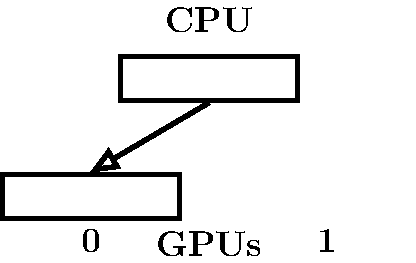
\includegraphics[width=\textwidth]{PaCT/singleDistribution_vector}
    \caption{\emph{single}}
    \label{fig:distributions:single}
  \end{subfigure}
  \hfill
  \begin{subfigure}{.3\textwidth}
    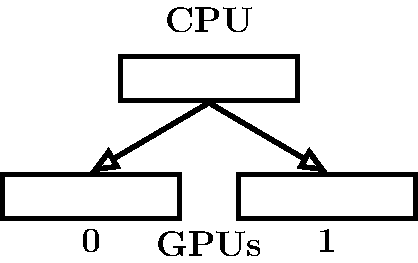
\includegraphics[width=\textwidth]{PaCT/copyDistribution_vector}
    \caption{\emph{copy}}
    \label{fig:distributions:copy}
  \end{subfigure}
  \hfill
  \begin{subfigure}{.3\textwidth}
    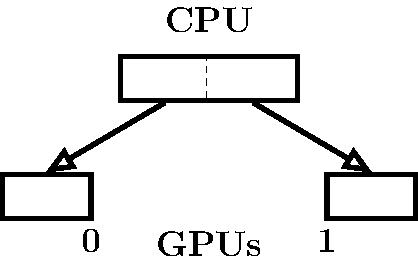
\includegraphics[width=\textwidth]{PaCT/blockDistribution_vector}
    \caption{\emph{block}}
    \label{fig:distributions:block}
  \end{subfigure}
  \caption{Distributions of a vector in SkelCL.}
  \label{fig:distributions}
  \bigskip
\end{figure}

\begin{figure}[tbp]
  \centering
  \begin{subfigure}{.22\textwidth}
    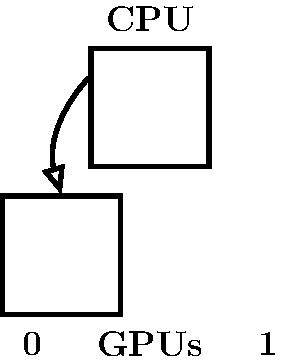
\includegraphics[width=\textwidth]{PaCT/singleDistribution_matrix}
    \caption{\emph{single}}
    \label{fig:distributions_matrix:single}
  \end{subfigure}
  \hfill
  \begin{subfigure}{.22\textwidth}
    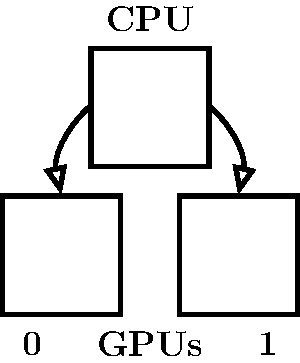
\includegraphics[width=\textwidth]{PaCT/copyDistribution_matrix}
    \caption{\emph{copy}}
    \label{fig:distributions_matrix:copy}
  \end{subfigure}
  \hfill
  \begin{subfigure}{.22\textwidth}
    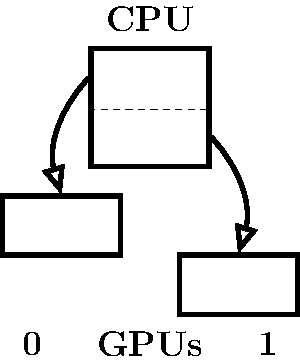
\includegraphics[width=\textwidth]{PaCT/blockDistribution_matrix}
    \caption{\emph{block}}
    \label{fig:distributions_matrix:block}
  \end{subfigure}
  \caption{Distributions of a matrix in SkelCL.}
  \label{fig:distributions_matrix}
\end{figure}


Three kinds of basic distributions are currently available in \SkelCL:
\emph{single}, \emph{copy}, and \emph{block} (see \autoref{fig:distributions} for distributing a vector on a system with two \GPUs).
If distribution is set to \emph{single} (\autoref{fig:distributions:single}), then vector's whole data is stored on a single \GPU (the first \GPU if not specified otherwise).
The \emph{copy} distribution (\autoref{fig:distributions:copy}) copies vector's entire data to each available \GPU.
With the \emph{block} distribution (\autoref{fig:distributions:block}), each \GPU stores a contiguous, disjoint chunk of the vector.

The same three distributions are provided also for the matrix data type as shown in \autoref{fig:distributions_matrix}.
The \emph{block} distribution (\autoref{fig:distributions_matrix:block}) splits the matrix into chunks of rows, which simplifies the implementation.

% In particular the overlap distribution splits the matrix into one chunk for each GPU; in addition, each chunk contains a number of continuous rows from the neighboring chunks.
% A parameter -- the \emph{overlap size} -- specifies the number of rows at the borders of a chunk which are copied to the two neighboring GPUs.
% \autoref{fig:Distribution_matrix:overlap} illustrates the overlap distribution:
% GPU 0 receives the top chunk ranging from the top row to the middle, while GPU 1 receives the second chunk ranging from the middle row to the bottom.
% The marked parts are called \emph{overlap region} they are the same on both GPUs.

The application developer can set the distribution of containers explicitly, otherwise every skeleton selects a default distribution for its input and output containers.
Container's distribution can be changed at runtime:
this implies data exchanges between multiple \GPUs and the \CPU, which are performed by the \SkelCL implementation implicitly.
As seen earlier in this chapter (\autoref{lst:lmosem:redistribution}) implementing such data transfers in the standard \OpenCL is a cumbersome task:
data has to be downloaded to the \CPU before it is uploaded to the \GPUs, including the corresponding length and offset calculations;
this results in a lot of low-level code which becomes completely hidden when using \SkelCL.

A special situation arises when the distribution is changed from the \emph{copy} distribution to any other distribution.
In this case each \GPU holds its own full copy of the data which might have been modified locally on each \GPU.
In order to maintain \SkelCL's concept of a self-contained container, these different versions are combined using a user-specified function when the distribution is changed.
If no function is specified, the copy of the first \GPU is taken as the new version of the container; the copies of the other \GPUs are discarded.


% ============================================================================ %
\subsection{More Complex Algorithmic Skeletons}
\label{section:skelcl-programming-model:specialSkeletons}

The basic algorithmic skeletons presented in~\autoref{section:skelcl-programming-model:skeletons} are long known in the functional and algorithmic skeleton communities.
In this section we will introduce two new more advanced algorithmic skeletons, which are more restrictive.
By limiting the use cases of these novel algorithmic skeleton we are able to make more assumptions in the implementation and provide advanced optimizations on modern multi-\GPU systems.

The first new skeleton (\stencil) is targeted towards \emph{stencil} (\aka nearest neighbor) computations, which are computations performed for every element of a container while including neighboring elements in the computation.
The second new skeleton (\allpairs) combines two matrix containers in an all-to-all fashion, which is a pattern used in applications like n-body simulation or matrix matrix multiplication.

For both skeletons we will first formally define them before looking at possible use cases.
Their implementations targeting multi-\GPU systems will be described in~\autoref{section:skelcl-library}.


\subsubsection{The \stencil Skeleton}

Many numerical and image processing applications dealing with two-dimensional data perform calculations for a particular data element taking neighboring data elements into account.
These type of applications are also known as \emph{stencil} or \emph{nearest neighbor} applications.
To facilitate the development of such applications, we introduce the \stencil skeleton that can be used with both vector and matrix data type.

The \stencil skeleton is customized with three parameters: a unary function $f$, an integer value $d$, and an out-of-bounds function $h$.
The skeleton applies $f$ to each element of an input container while taking the neighboring elements within the range $d$ in each dimension into account.
When neighboring elements are accesses at the boundaries of the container out of bound accesses occur.
In these cases the function $h$ is called with the index causing the out of bound access and should return a replacement value.
We now formally define the \stencil skeleton. We start with the definition for vectors:
\begin{definition}
  \label{definition:mapoverlap}
  Let $\vec{x}$ be a vector of size $n$ with elements $x_i$ where $0 < i \leq n$.
  Let $f$ be a customizing function, $d$ be a positive integer value, and $h$ be an out-of-bound handling function.
  The algorithmic skeleton \stencil is defined as follows:
  \begin{equation*}
    \begin{split}
    &\stencil\ f\  d\ h\ [x_1, x_2, \ldots, x_n] \eqdef [y_1, y_2, \dots, y_n]\\
    &\text{where}\\[.5em]
    &\qquad y_i = f\ [x_{i-d}, \ldots, x_{i+d}] \qquad \forall\ i :  0 < i \leq n\\
    &\text{and\hfill}\\
    &\qquad x_j = h\ j \qquad \forall\ j : -d < j \leq 0\ \vee n < j \leq n+d
    \end{split}
  \end{equation*}
\end{definition}

\noindent
The definition for matrices is similar:
\begin{definition}
  \label{definition:mapoverlap:matrix}
  Let $M$ be an $n\times m$ matrix with elements $m_{i,j}$ where $0 < i \leq n$ and $0 < j \leq m$.
  Let $f$ be a customizing function, $d$ be an positive integer value, and $h$ be a out of bound handling function.
  The algorithmic skeleton \stencil is defined as follows:
  \begin{equation*}
    \begin{split}
    & \stencil\ f\  d\ h\ \DottedMatrix{m_{0,0}}{m_{0,m}}{m_{n,0}}{m_{n,m}}
               \eqdef \DottedMatrix{n_{0,0}}{n_{0,m}}{n_{n,0}}{n_{n,m}}\\
               &\text{where}\\[.5em]
    &\qquad n_{i,j} = f\ \DottedMatrix{m_{i-d,j-d}}{m_{i-d,j+d}}{m_{i+d,j-d}}{m_{i+d,j+d}} \qquad \forall\ i,j
        \begin{array}{r} 0 < i \leq n,\\ 0 < j \leq m \end{array}\\
        &\text{and}\\
    &\qquad m_{i,j} = h\ i\ j \qquad \forall\ i,j \begin{array}{r} -d < j \leq 0\ \vee n < j \leq n+d,\\ -d < j \leq 0\ \vee m < j \leq m+d \end{array}
    \end{split}
  \end{equation*}
\end{definition}


SkelCL currently supports a fixed set of choices for the out-of-bound handling function $h$ motivated by common cases of of bound handling in image processing applications.
This restriction could easily be lifted in the future.
The \stencil skeleton can currently be configured to handle out of bound accesses in two possible ways:
\begin{enumerate}
  \item a specified neutral value is returned (\ie, the out of bound function $h$ is constant);
  \item the nearest valid value inside the container is returned.
\end{enumerate}

Possible applications for the \stencil skeleton are image processing applications or physics simulations (see~\autoref{sec:imageProcessing} and \autoref{sec:physicsSim}).
A simple example application is the \emph{discrete Laplacian operator} used in image processing, \eg, for edge detection~\cite{Umbaugh1997}.
It computes a new value for every pixel of an image by weighting and summing up its direct neighboring pixel values, as follows:
\begin{align*}
  laplacian&\ M = \stencil\ f\ 1\ \overline{0}\ M\\
  \text{where:} \ \ &
  \begin{array}{ll}%
  f&\ \left[\begin{array}{ccc}%
      \hspace{-.5em} m_{i-1,j-1}& \hspace{-.5em} m_{i-1,j} & \hspace{-.5em}m_{i-1,j+1}\vspace{-.25em}\\%
      \hspace{-.5em} m_{i,j-1}  & \hspace{-.5em} m_{i,j}   & \hspace{-.5em}m_{i,j+1}  \vspace{-.25em}\\%
      \hspace{-.5em} m_{i+1,j-1}& \hspace{-.5em} m_{i+1,j} & \hspace{-.5em}m_{i+1,j+1}
    \end{array}\right] = \\[2em]
          &\ m_{i-1,j} + m_{i,j-1} - 4 \times m_{i,j} + m_{i,j+1} + m_{i+1,j}
  \end{array} \\
  \text{and } \overline{0} \text{ is th}&\text{e constant function always returning 0.}
\end{align*}

\subsubsection{The overlap data distribution}

\begin{figure}[tb]
  \centering
  \begin{subfigure}[b]{.3\textwidth}
    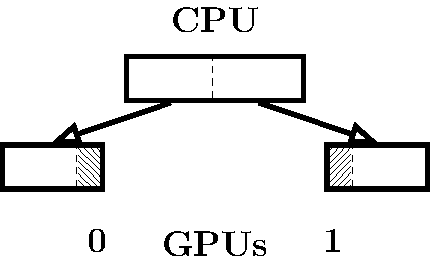
\includegraphics[width=\textwidth]{PaCT/overlapDistribution_vector}
    \caption{\emph{overlap}}
    \label{fig:overlap_distribution}
  \end{subfigure}
  \hspace{3em}
  \begin{subfigure}[b]{.22\textwidth}
    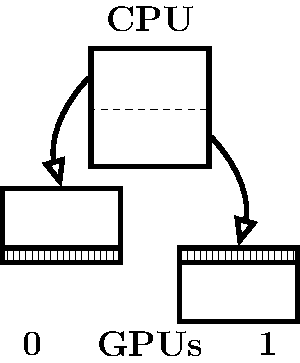
\includegraphics[width=\textwidth]{PaCT/overlapDistribution_matrix}
    \caption{\emph{overlap}}
    \label{fig:overlap_distribution:matrix}
  \end{subfigure}
  \caption{Overlap distribution of a vector and matrix in SkelCL.}
  \label{fig:overlap_distribution}
  \bigskip
\end{figure}

Together with the \stencil skeleton we introduce a new distribution called \emph{overlap} (Figure~\ref{fig:overlap_distribution}).
The overlap distribution splits the container into one chunk for each device, similarly to the \emph{block} distribution.
In addition, each chunk consists of a number of continuous elements (in case of the vector) or rows (in case of the matrix) which are copied to the neighboring devices, similar to the \emph{copy} distribution.
Therefore, the overlap distribution can be seen as a combination of the \emph{block} and \emph{copy} distribution.
The number of elements or rows at the edges of a chunk which are copied to the neighboring devices are called the \emph{overlap size}.

The \emph{overlap} distribution ensures that neighboring elements are always accessible even if the container is split across multiple devices.
The \emph{overlap} distribution is, therefore, automatically selected as distribution by the \stencil skeleton automatically setting the overlap size to the skeleton parameter $d$, which ensures that every device has access to the necessary neighboring elements.





\subsubsection{The \allpairs Skeleton}
\label{sec:allpairs_skeleton}

\emph{Allpairs computations} occur in a variety of applications, ranging from matrix multiplication and N-Body simulations in physics~\cite{AroraShVu2009} to pairwise Manhattan distance computations in bioinformatics~\cite{ChangDeQuRo2009}.
These applications share a common computational pattern:
for two sets of entities, the same computation is performed independently for all pairs in which entities from the first set are combined with entities from the second set.
We define the \allpairs skeleton to simplify the development of such applications.
We represent the entries of both sets as vectors of length $d$, where the cardinality of the first set is $n$ and the cardinality of the second set is $m$.
We model the first set as a $n\times d$ matrix $A$ and the second set as a $m\times d$ matrix $B$.
The allpairs computation yields an output matrix $C$ of size $n\times m$ with $c_{i, j} = a_i \oplus b_j$, where $a_i$ and $b_j$ are row vectors of $A$ and $B$, correspondingly,
%:
%$a_i = [a_{i,1}, \cdots, a_{i, d}]$, $b_j = [b_{j,1}, \cdots, b_{j,d}]$,
and $\oplus$ is a binary operator defined on vectors.

We formally define the \allpairs skeleton as follows:

\begin{definition}
  \label{def:allpairs}
  Let $A$ be a $n\times d$ matrix, $B$ be a $m\times d$ matrix, and $C$ be a $n\times m$ matrix, with their elements $a_{i,j}$, $b_{i,j}$, and $C_{i,j}$ respectively.
  The algorithmic skeleton \allpairs with customizing binary function $\oplus$ is defined as follows:
  \begin{equation*}
    \begin{split}
    allpairs\ (&\oplus)\
      \left[ \begin{array}{ccc} a_{1,1} & \cdots & a_{1,d}\\[.25em] \vdots & & \vdots\\[.25em] a_{n,1} & \cdots & a_{n,d} \end{array}\right]\ %
      \left[ \begin{array}{ccc} b_{1,1} & \cdots & b_{1,d}\\[-.25em] \cdot & & \cdot\\[-.75em] \cdot & & \cdot\\[-.25em] b_{m,1} & \cdots & b_{m,d} \end{array}\right]%
      \\
    &\eqdef \left[ \begin{array}{ccc} C_{1,1} & \cdots & C_{1,m}\\[.25em] \vdots & & \vdots\\[.25em] C_{n,1} & \cdots & C_{n,m} \end{array} \right]
    \end{split}
  \end{equation*}
  where elements $C_{i,j}$ of the $n\times m$ matrix $C$ are computed as follows:
  \[
    C_{i,j} = \DottedVector{a_{i,1}}{a_{i,d}} \oplus \DottedVector{b_{j,1}}{b_{j,d}}
  \]
\end{definition}

\autoref{fig:allpairs:access:not_transposed} illustrates this definition:
the element $C_{2,3}$ of matrix $C$ marked as \circled{3} is computed by combining the second row of $A$ marked as \circled{1} with the third row of $B$ marked as \circled{2} using the binary operator $\oplus$.
\autoref{fig:allpairs:access:transposed} shows the same computation with the transposed matrix $B$.
This visualization shows how the structure of matrix $C$ is determined by the two input matrices $A$ and $B$.

\begin{figure}[tb]
  \centering
  \begin{subfigure}[b]{.44\textwidth}
    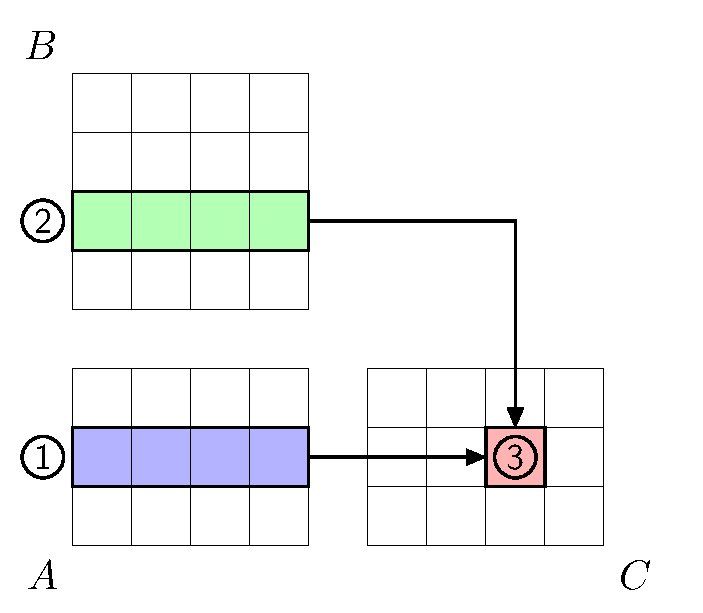
\includegraphics[width=\textwidth]{HLPP/allpairs_access_pattern_alternative}
    \caption{}
    \label{fig:allpairs:access:not_transposed}
  \end{subfigure}
  \hfill
  \begin{subfigure}[b]{.44\textwidth}
    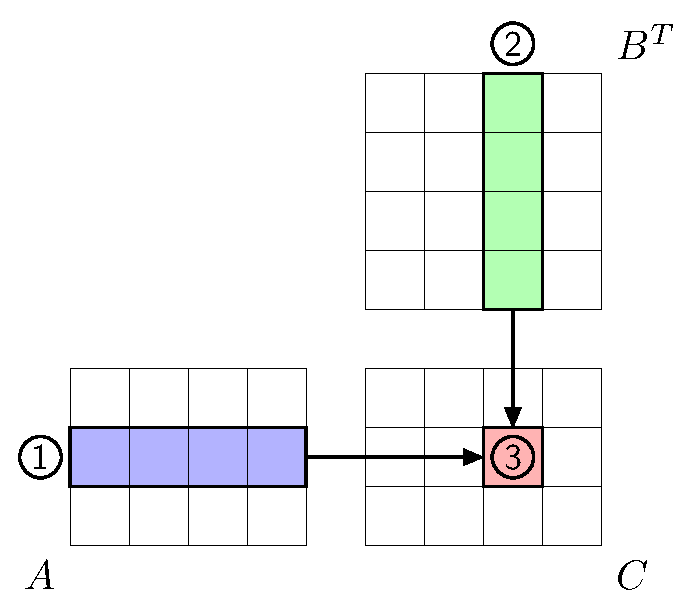
\includegraphics[width=\textwidth]{HLPP/allpairs_access_pattern}
    \caption{}
    \label{fig:allpairs:access:transposed}
  \end{subfigure}
  \caption{The allpairs computation schema. (\subref{fig:allpairs:access:not_transposed}): element $C_{2,3}$
    \protect\tikz[baseline=(char.base)]\protect\node[shape=circle,draw,inner sep=1pt] (char) {3};
    is computed by combining the second row of $A$
    \protect\tikz[baseline=(char.base)]\protect\node[shape=circle,draw,inner sep=1pt] (char) {1};
    with the third row of $B$
    \protect\tikz[baseline=(char.base)]\protect\node[shape=circle,draw,inner sep=1pt] (char) {2};
    using the binary operator $\oplus$. (\subref{fig:allpairs:access:transposed}): the same situation where the transpose of matrix $B$ is shown.}
  \label{fig:allpairs:access}
\end{figure}

Let us consider two example applications which can be expressed by customizing the \allpairs skeleton with a particular function $\oplus$.

\paragraph{Example 1:}
The Manhattan distance (or $L_1$ distance) is a measure of distance which is used in many applications.
In general, it is defined for two vectors, $x$ and $y$, of equal length $d$, as follows:
\begin{equation}
  \label{eq:man_dist}
  \ManDist\ x\ y = \sum_{k=1}^d | x_k - y_k |
\end{equation}
In~\cite{ChangDeQuRo2009}, the so-called Pairwise Manhattan Distance (\emph{PMD}) is studied as a fundamental operation in hierarchical clustering for data analysis.
\emph{PMD} is obtained by computing the Manhattan distance for every pair of rows of a given matrix.
This computation for arbitrary matrix $A$ can be expressed using the \allpairs skeleton customized with the Manhattan distance defined in \autoref{eq:man_dist}:
\begin{equation}
  \PMD\ A = allpairs\ \mbox{\emph{ManDist}}\ A\ A
\end{equation}
The $n\times n$ matrix computed by the customized skeleton contains the Manhattan distance for every pair of rows of the input $n\times d$ matrix $A$.

\paragraph{Example 2:}
Matrix-matrix multiplication is a basic linear algebra operation, which is a building block of many scientific applications.
A $n\times d$ matrix $A$ is multiplied with a $d\times m$ matrix $B$, producing a $n\times m$ matrix $C=A\times B$ whose element $C_{i,j}$ is computed as the dot product of the $i$th row of $A$ with the $j$th column of $B$.
The dot product of two vectors, $a$ and $b$ of length $d$, is computed as follows:
\begin{equation}
  \dotProduct\ a\ b = \sum_{k=1}^d a_k \cdot b_k
\end{equation}
The matrix multiplication can be expressed using the \allpairs skeleton as:
\begin{equation}
  A\times B = allpairs\ \dotProduct\ A\ B^T
  \label{eq:mat_mult_allpairs}
\end{equation}
where $B^T$ is the transpose of matrix $B$.

% TODO: moved to impl ...
% \paragraph{The \allpairs skeleton using multiple GPUs}
% \label{sec:allpairs:multi_gpu}
% \begin{figure}[b]
%   \centering
%   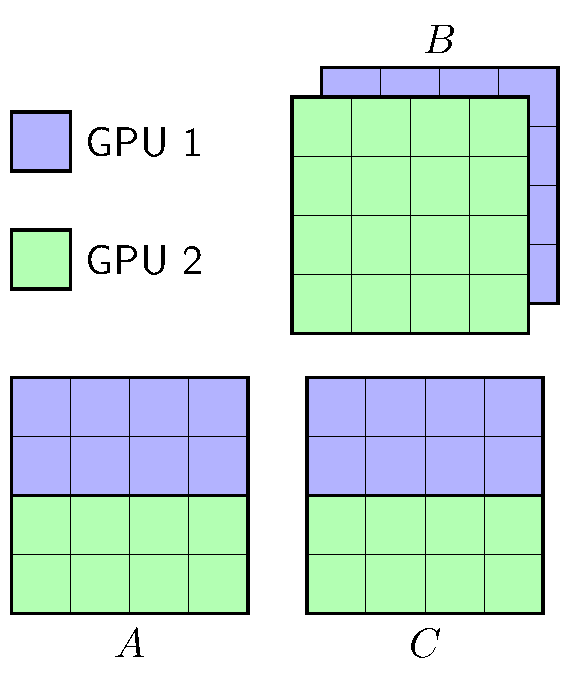
\includegraphics[width=.3\textwidth]{HLPP/multi_gpu}
%   \caption{Data distributions used for a system with two GPUs: matrices $A$ and $C$ are \emph{block} distributed, matrix $B$ is \emph{copy} distributed.}
%   \label{fig:multi_gpu}
% \end{figure}
% 
% The \allpairs skeleton can be efficiently implemented not only on systems with a single \GPU, but on multi-\GPU systems as well.
% The necessary data distribution can be easily expressed using two of \SkelCL's \emph{distributions}, as shown in \autoref{fig:multi_gpu}:
% Matrix $B$ is \emph{copy} distributed, \ie, it is copied entirely to all \GPUs in the system.
% Matrix $A$ and $C$ are \emph{block} distributed, \ie, they are row-divided into as many equally-sized blocks as \GPUs are available;
% each block is copied to its corresponding \GPU.
% Following these distributions, each \GPU computes one block of the result matrix $C$.
% In the example with two GPUs shown in \autoref{fig:multi_gpu}, the first two rows of $C$ are computed by \GPU 1 and the last two rows by \GPU 2.
% The \allpairs skeleton automatically selects these distributions, therefore, the same source code can be used when using a single \GPU or multiple \GPUs.



\subsubsection{The specialized \allpairs skeleton}
\label{sec:opt_allpairs_skeleton}
When targeting \GPU architectures, implementing an optimized version of the \allpairs skeleton is possible if certain assumptions about the customizing function $f$ can be made.
In this section, we will start by discussing the properties of $f$ necessary for an optimized \GPU implementation.
In particular we will analyze the memory access pattern of the matrix multiplication as the memory accesses turns out to be crucial for the performance.
We then observe that the identified memory access pattern can also be found in other allpairs computations and, therefore, define a specialized version of the allpairs skeleton, which is suitable for applications having this pattern.
% Finally, we estimate the gained efficiency by the optimized implementation over the generic one.


\paragraph{The memory access pattern of the matrix multiplication}
\begin{figure}[t]
  \centering
  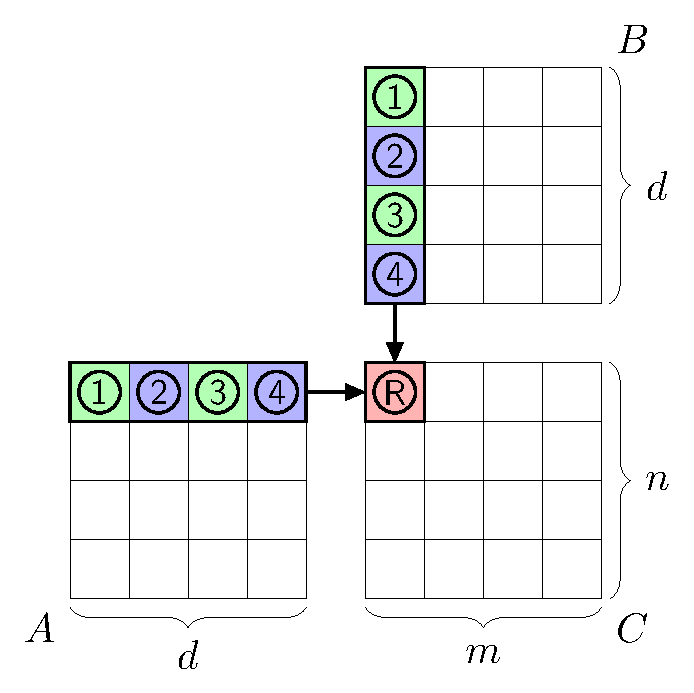
\includegraphics[width=0.4\textwidth]{HLPP/single_memory_access}
  \caption{The memory access pattern of the matrix multiplication $A\times B = C$.}
  \label{fig:mm_access_pattern}
\end{figure}
Figure~\ref{fig:mm_access_pattern} shows the memory access pattern of the matrix multiplication for $4\times 4$ matrices.
To compute the element \circled{R} of the result matrix $C$, the first row of matrix $A$ and the first column of matrix $B$ are combined.
In the skeleton-based code, these two vectors are used by the customizing function $f$, which is the dot product in case of the matrix multiplication.
The dot product performs a pairwise multiplication of the two vectors and then sums up the intermediate result.
In the example, the two elements marked as \circled{1} are multiplied first and the intermediate result is stored;
then, the next elements (marked as \circled{2}) are multiplied and the result is added to the intermediate result, and so forth.
% TODO: Moved to impl section ...
% Let us assume targeting \GPU architectures and estimate the number of global (and therefore expensive) memory accesses required for computing an element of the matrix multiplication in the generic case.
% One global memory read access for every element of both input vectors is performed, and a single global memory write access is required to write the result into the output matrix.
% Therefore, 
% \begin{equation}
%   n\cdot m\cdot (d + d + 1)
%   \label{eq:mm:accesses}
% \end{equation}
% global memory accesses are performed in total, where $n$ and $m$ are the height and width of matrix $C$ and $d$ is the width of $A$ and the height of $B$.
% By using the fast but small local memory this number of global memory accesses can be reduces and, thus, performance can be improved.
% Using the local memory for matrix matrix multiplication is a well known optimization.

A key observation is, that other applications share the same memory access pattern as the matrix multiplication shown in \autoref{fig:mm_access_pattern}.
For example, the customizing function of the pairwise Manhattan distance as defined by \autoref{eq:man_dist} follows obviously the same memory access pattern as the matrix multiplication.
To find a common representation for a customizing function with this pairwise access pattern, we describe it as a sequential composition of two basic algorithmic skeletons: \zip and \reduce.
% The \emph{sequential composition} composition of two functions (or skeletons) $f$ and $g$ is denoted by $g \circ f$ which means that $f$ is applied first and then $g$ is applied to the result value of $f$ as input, \ie, $(g\circ f)\ x = g(f\ x)$.

For the \reduce skeleton customized with $\oplus$ and corresponding identity element \id, and the \zip skeleton customized with $\otimes$ we can sequentially compose them as follows:
\begin{eqnarray*}
  \reduce\ (\oplus)\ \id\ \big(\ \zip\ (\otimes)\ a\ b\ \big) &=&\\
  \reduce\ (\oplus)\ \id\ \big(\ \zip\ (\otimes)\ \DottedVector{a_1}{a_n}\ \DottedVector{b_1}{b_n}\ \big) &=&\\
  (a_1 \otimes b_1)\ \ \oplus &\cdots& \oplus\ \ (a_n \otimes b_n)
\end{eqnarray*}

This composition of the two customized skeletons yields a function which we denote \zipReduce; it takes two input vectors and produces a single scalar value:

\begin{equation*}
  \zipReduce\ (\oplus)\ \id\ (\otimes)\ a\ b \eqdef 
  \reduce\ (\oplus)\ \id\ \big(\ \zip\ (\otimes)\ a\ b\ \big)
\end{equation*}

Following the definition of \zipReduce, we can express the customizing function of the Manhattan distance as follows.
We use the binary operator $a \ominus b = |a - b|$ as the customizing function for \zip, and addition as the customizing function for the \reduce skeleton:
\begin{eqnarray*}
    \ManDist\ a\ b &=& \sum_{i=1}^{n} | a_i - b_i | = (a_1 \ominus b_1) + \cdots + (a_n \ominus b_n)\\
    &=& \zipReduce\ (+)\ 0\ (\ominus)\ \DottedVector{a_1}{a_n}\ \DottedVector{b_1}{b_n}
\end{eqnarray*}

Similarly, we can express the dot product (which is the customizing function of matrix multiplication) as a \zip-\reduce composition, by using multiplication for customizing the \zip skeleton and addition for customizing the \reduce skeleton:
\begin{eqnarray*}
  \dotProduct\ a\ b &=& \sum_{i = 1}^{n} a_i \cdot b_i = (a_1 \cdot b_1) + \cdots + (a_n \cdot b_n)\\
  &=& \zipReduce\ (+)\ 0\ (\times)\ a\ b
\end{eqnarray*}

\paragraph{Definition of the specialized \allpairs skeleton}

We can now specialize the generic Definition~\autoref{def:allpairs} of the \allpairs skeleton by employing the sequential composition of the customized \reduce and \zip skeletons for customizing the \allpairs skeleton.
From here on, we refer to this specialization as the \allpairs skeleton \emph{customized with \zip-\reduce}.

\begin{definition}
  \label{def:allpairs:specialized}
  Let $A$ be a $n\times d$ matrix, $B$ be a $m\times d$ matrix, and $C$ be a $n\times m$ matrix, with their elements $a_{i,j}$, $b_{i,j}$, and $C_{i,j}$ respectively.
  Let $\oplus$ be an associative binary customizing operator with the corresponding identity element \id.
  Let $\otimes$ be a binary customizing operator.
  The specialized algorithmic skeleton \allpairs customized with \zip-\reduce is defined as follows:
  \begin{equation*}
    \begin{split}
      \allpairs\ (\oplus)\ \id\ (&\otimes)\ %
      \left[ \begin{array}{c} a_{1,1} \cdots a_{1,d}\\[.25em] \vdots \hspace{4em} \vdots\\[.25em] a_{n,1} \cdots a_{n,d} \end{array}\right]\ %
      \left[ \begin{array}{c} b_{1,1} \cdots b_{1,d}\\[-.25em] \cdot \hspace{4em} \cdot\\[-.75em] \cdot \hspace{4em} \cdot\\[-.25em] b_{m,1} \cdots b_{m,d} \end{array}\right]%
      \\
    &\eqdef \left[ \begin{array}{ccc} C_{1,1} & \cdots & C_{1,m}\\[.25em] \vdots & & \vdots\\[.25em] C_{n,1} & \cdots & C_{n,m} \end{array} \right]
    \end{split}
  \end{equation*}
  where elements $C_{i,j}$ of the $n\times m$ matrix $C$ are computed as follows:
  \[
    C_{i,j} = \zipReduce\ (\oplus)\ \id\ (\otimes)\ \DottedVector{a_{i,1}}{a_{i,d}}\ \DottedVector{b_{j,1}}{b_{j,d}}
  \]
\end{definition}


While not every allpairs computation can be expressed using this specialization, many real-world problems can.
In addition to the matrix multiplication and the pairwise Manhattan distance examples are the pairwise computation of the Pearson correlation coefficient~\cite{ChangDeQuRo2009} and estimation of Mutual Informations~\cite{DaubStSeKl2004}.
The composition of \zip and \reduce is well known in the functional programming world.
Google's popular \emph{MapReduce} programming model has been inspired by a similar composition of the \map and \reduce skeletons.
\cite{Laemmel2007} extensively discusses the relation of MapReduce to functional programming.


% TODO: Moved to impl ...
% \paragraph{Estimation of the performance gain of specialization}
% By expressing the customizing function of the \allpairs skeleton as a \zip-\reduce composition, we provide additional semantic information about the memory access pattern of the customizing function to the skeleton implementation, thus allowing for improving the performance.
% Our idea of optimization is based on the OpenCL programming model that organizes \emph{work-items} (i.\,e., threads executing a kernel) in \emph{work-groups} which share the same \GPU local memory.
% By loading data needed by multiple work-items of the same work-group into the local memory, we can avoid repetitive accesses to the global memory.
% 
% \begin{figure}[b]
%   \centering
%   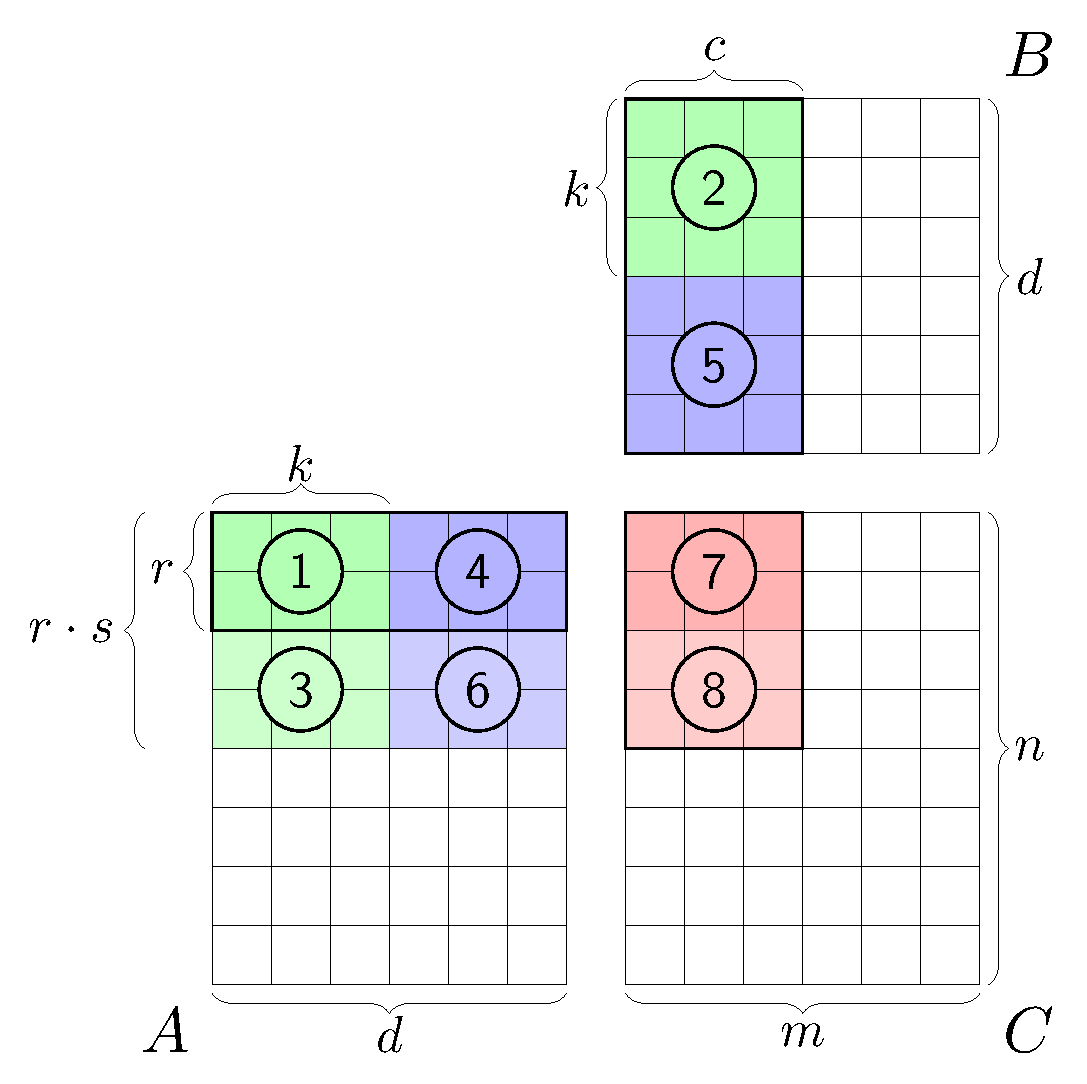
\includegraphics[width=.4\textwidth]{HLPP/memory_access}
%   \caption{Implementation schema of the specialized allpairs skeleton.}
%   \label{fig:memory_access}
% \end{figure}
% For the \allpairs skeleton with the \zip-\reduce customizing function, we can adopt the implementation schema for \GPUs~\cite{SarjeAl2013}, as shown in Figure~\ref{fig:memory_access}.
% We allocate two arrays in the local memory, one of size $r\times k$ ($r=2$, $k=3$ in Figure~\ref{fig:memory_access}) for elements of $A$ and one of size $k\times c$ ($c=3$ in Figure~\ref{fig:memory_access}) for elements of $B$.
% A work-group consisting of $c\times r$ work-items computes $s$ blocks ($s=2$ in Figure~\ref{fig:memory_access}) of the result matrix $C$.
% In Figure~\ref{fig:memory_access}, the two blocks marked as \circled{7} and \circled{8} are computed by the same work-group as follows.
% In the first iteration, the elements of blocks \circled{1} and \circled{2} are loaded into the local memory and combined following the \zip-\reduce pattern.
% The obtained intermediate result is stored in block \circled{7}.
% Then, the elements of block \circled{3} are loaded and combined with the elements from \circled{2} which still reside in the local memory.
% The intermediate result is stored in block \circled{8}.
% In the second iteration, the algorithm continues in the same manner with blocks \circled{4}, \circled{5}, and \circled{6}, but this time, the elements of the blocks are also combined with the intermediate results of the first iteration, which are stored in blocks \circled{7} and \circled{8}.
% The advantage of computing multiple blocks by the same work-group is that we keep the elements of $B$ in the local memory when computing the intermediate results, \ie, we do not reload block \circled{2} twice for the computation of blocks \circled{7} and \circled{8}.
% 
% Every element loaded from the global memory is used by multiple work-items:
% \eg, the upper left element of block \circled{1} is loaded only once from the global memory, but used three times:
% in the computation of the upper left, upper middle, and upper right elements of \circled{7}.
% In general, every element loaded from $A$ is reused $c$ times, and every element from $B$ is reused $r\cdot s$ times.
% As the intermediate results are stored in the global memory of matrix $C$, we perform two additional memory accesses (read/write) for every iteration, \ie, $2\cdot \frac{d}{k}$ in total.
% Therefore, instead of $n\cdot m\cdot (d + d + 1)$ (see \autoref{eq:mm:accesses}) global memory accesses necessary when using the non-specialized skeleton and, thus, only the global memory, only
% \begin{equation}
%   n\cdot m\cdot (\frac{d}{r\cdot s} + \frac{d}{c} + 2\cdot \frac{d}{k})
% \end{equation}
% global memory accesses are performed.
% By increasing the parameters $s$ and $k$, or the number of work-items in a work-group ($c$ and $r$), more global memory accesses can be saved.
% However, the work-group size is limited by the \GPU hardware.
% While the parameters can be chosen independently of the matrix sizes, we have to consider the amount of available local memory.
% \cite{Friese2013}~and~\cite{SarjeAl2013}~discusses how suitable parameters can be found by performing runtime experiments.
% In~\cite{Friese2013} the parameters $c = 32$, $r=8$, $s=32$, and $k=64$ are used on modern \GPU hardware showing good performance.
% 
% We will report measurements of the performance difference for the two skeleton implementations on real hardware in \autoref{chapter:skelcl:apps}.
% 
% 




% ============================================================================ %
% ============================================================================ %
\section{The \SkelCL Library}
\label{section:skelcl-library}
In this section we discuss the \SkelCL library -- our implementation of the \SkelCL programming model.
It provides a \Cpp~\API that implements the features of the \SkelCL programming model, and thus liberates the application developer from writing low-level code.
In addition, the library provides some commonly used utility functions, \eg, for program initialization.
The \SkelCL library is open source software and available at: \url{http://skelcl.uni-muenster.de}.

We start our discussion with an example showing how to use the \SkelCL library.
We describe the syntax used to represent the \SkelCL programming model introduced in the previous section.
This will include a discussion of \Cpp techniques used to implement the library.
We then shift the focus to the implementations of the memory management, algorithmic skeletons, and distributions.










\subsection{Programming with the \SkelCL Library}

\autoref{lst:skelcl:dotproduct} shows the implementation of the dot product computation, discussed in the previous section, in \SkelCL.
After including the appropriate \SkelCL headers (\autoref{lst:skelcl:dotproduct:inc:start}---\autoref{lst:skelcl:dotproduct:inc:end}) the \SkelCL library can be initialized as shown in \autoref{lst:skelcl:dotproduct:init}.
This will perform the initializations required by \OpenCL.
The argument provided to the \code{init} function specifies how many and which \OpenCL devices should be used by \SkelCL.
Here a single device should be used which can be of any type, \ie, it can be either a \CPU or a \GPU.
The dot product is specified using the \zip and \reduce skeletons.
The skeletons are created using \code{zip} (\autoref{lst:skelcl:dotproduct:zip}) and \code{reduce} (\autoref{lst:skelcl:dotproduct:reduce}) functions which expect the customizing functions of the skeletons as arguments.
In this example we use \Cpp lambda expressions (\autoref{lst:skelcl:dotproduct:zip:lambda} and \autoref{lst:skelcl:dotproduct:reduce:lambda}) to specify the customizing functions of the skeletons.
We create the two input \code{Vector}s from C style pointers (\autoref{lst:skelcl:dotproduct:vecAB}).
In \autoref{lst:skelcl:dotproduct:apply} we perform the computation by applying the customized skeletons to the data, before we finally return the computed result in \autoref{lst:skelcl:dotproduct:return}.

\begin{lstlisting}[%
caption={Implementation of the dot product computation in \SkelCL.},%
float=t,%
numbers=left,%
label={lst:skelcl:dotproduct}]
#include <SkelCL/SkelCL.h>$\label{lst:skelcl:dotproduct:inc:start}$
#include <SkelCL/Zip.h>
#include <SkelCL/Reduce.h>
#include <SkelCL/Vector.h>$\label{lst:skelcl:dotproduct:inc:end}$

float dotProduct(const float* a, const float* b, int n) {
  using namespace skelcl;
  skelcl::init( 1_device.type(deviceType::ANY) );$\label{lst:skelcl:dotproduct:init}$

  auto mult = zip([](float x, float y) { return x*y; });$\label{lst:skelcl:dotproduct:zip}$$\label{lst:skelcl:dotproduct:zip:lambda}$
  auto sum = reduce([](float x, float y){ return x+y; }, 0);$\label{lst:skelcl:dotproduct:reduce}$$\label{lst:skelcl:dotproduct:reduce:lambda}$

  Vector<float> A(a, a+n); Vector<float> B(b, b+n);$\label{lst:skelcl:dotproduct:vecAB}$

  Vector<float> C = sum( mult(A, B) );$\label{lst:skelcl:dotproduct:apply}$

  return C.front();$\label{lst:skelcl:dotproduct:return}$
}
\end{lstlisting}

\autoref{lst:skelcl:dotproduct} shows that the \SkelCL library integrates nicely with \Cpp:
the interface of the \code{Vector} class looks familiar to \Cpp programmers and the usage of modern \Cpp features like lambda expressions, type deduction (\code{auto}), and user-defined literals simplify the programming as functions can be defined directly inline, type information can be omitted, and the specification of which devices to use can be written intuitively.

We will now discuss how our implementation enables this comfortable level of integrating \SkelCL with \Cpp.










\subsection{Syntax and Integration with \Cpp}
\label{section:skelcl-library:syntax}

The \SkelCL library is built on top of \OpenCL.
This offers clear benefits as well as introduces technical challenges.
One of the technical challenges is, that \OpenCL requires the kernel to be specified as a string in the host program.
While this enables portability across different hardware architectures, it also introduces a burden on the application developer as strong typing cannot be guaranteed statically when the host program is compiled.
For the implementation of \SkelCL, we choose to address this issue using a two-step implementation.
In the first step, a custom compiler transforms the source code as seen in \autoref{lst:skelcl:dotproduct} to a representation where the kernel computations are represented as strings as required by \OpenCL.
In the second step, the transformed program is compiled using a traditional \Cpp compiler to produce the final executable.

This allows ourselves to free the users from writing strings in their application code and maintain the usual type safety guarantees from \Cpp at compile time.
Furthermore, we implemented type inference capabilities in our source-to-source compiler to free the application developer from specifying type information explicitly.
Our two-step design also allows application developers to compile their application code into a form which then can be deployed on systems where it might be difficult to install a custom compiler.

In the next paragraph, we will start the discussion of our source-to-source compiler.
We will discuss how our custom compiler, together with our template-based implementation, helps to maintain strong type safety at compile time.
Finally, we will look at issues regarding the integration with \Cpp like sharing code between host and device code.

\paragraph{The custom SkelCL compiler}
To allow a deep integration of \SkelCL code with \Cpp, we implemented a custom compiler: \code{skelclc}.
We leverage the LLVM infrastructure~\cite{Lattner2004} for building this compiler.
LLVM and the related Clang project offer well-defined application programming interfaces for writing C and \Cpp related compiler tools.
In particular the \emph{LibTooling} \API allows for writing tools which search for particular patterns in the abstract syntax tree (AST) which is representing the source code and perform actions on the found code fragments.
The \code{skelclc} custom compiler does exactly this.
For example, the custom compiler searches for an expression like this:
\begin{lstlisting}[numbers=none,label={lst:skelclc:before},caption={\SkelCL code snippet before transformation.}]
auto mult = zip( [](float x, float y){ return x*y; } );
\end{lstlisting}
and replaces it with:
\smallskip
\begin{lstlisting}[numbers=none,label={lst:skelclc:after},caption={\SkelCL code snippet after transformation.}]
auto mult = Zip<Container<float>(Container<float>,
                                 Container<float>)>(
              Source("float func(float x, float y)"
                     " { return x*y; }"), "func");
\end{lstlisting}

In this example, the \code{zip} function has been transformed into a call of the constructor of the \code{Zip} class and the lambda expression has been transformed into a string.
Furthermore, type information that has been inferred from the lambda expression, has been added to the templated \code{Zip} class.

The user is free to write the expression in \autoref{lst:skelclc:after} explicitly, but it is arguably more convenient to write the expression as in \autoref{lst:skelclc:before} and let \code{skelclc} perform the transformation automatically.

For every skeleton available in \SkelCL, there exists a function like \code{zip} which is transformed by \code{skelclc} to a call of the constructor of the corresponding skeleton class.

\paragraph{Maintaining type safety}
Each skeleton is represented by a templated class, as seen in \autoref{lst:skelclc:after} for the \zip skeleton.
The template arguments of the skeleton define the types which can be used when executing the skeleton.
For a skeleton of type \code{skeleton<T(U)>}, an object of type \code{U} has to be provided on execution to receive an object of type \code{T}.
In this respect skeletons behave exactly like functions in \Cpp which can be represented using the \code{std::function<T(U)>} template class.
Skeletons taking more then one argument (like the \code{zip} skeleton) are represented as \code{skeleton<T(U, V)>}.% using the \emph{variadic template} feature of \Cpp.

When performing the transformations, \code{skelclc} infers the types used as template arguments of the skeleton class.
To do so, it determines the types of the lambda expression arguments and skeleton's result type.
For \autoref{lst:skelclc:before} this is: \code{float} and \code{float} as argument types and \code{float} as the result type.
The result type is inferred following standard \Cpp rules.
Based on these types, the template arguments of the skeleton are constructed.

The skeletons \map, \zip, and \stencil can operate on either \code{Vector} or \code{Matrix}.
For each of these skeletons there exist three kinds of factory functions:
1)~for creating a skeleton operating on vectors, \eg, \code{mapVector};
2)~for creating a skeleton operating on matrices, \eg, \code{mapMatrix};
3)~for creating a skeleton capable of operating on both vectors and matrices, \eg, \code{map}.
To allow the latter case, the templated class \code{Container} was introduced.
Using the template specialization mechanism, the mentioned skeletons have a special implementation when \code{Container} is used as a template argument.
In this case, the classes provide a templated function call operator which can be used either with \code{Vector} or \code{Matrix}.

Type safety is guaranteed, as the templated skeleton classes can only be executed with a container of compatible type and the type inference ensures that the user function has exactly the same type as the template argument of the skeleton class.
Therefore, applying the user function to the input data is always a type-safe operation.

Because skeletons are strongly typed, the composition of skeletons is type-safe as well, \ie, in \autoref{lst:skelcl:dotproduct} type safety between the two skeletons is guaranteed.
If the result type of \code{zip} does not match the input type of \code{reduce}, a compile time error would occur.

\paragraph{Integration with \Cpp}
To allow a deep integration with \Cpp, a customizing function is allowed to make use of user-defined types and make calls to other functions.
The \code{skelclc} compiler detects these behaviors and ensures that the definition of the user defined type and the source code of all called functions is included in the source code passed to the skeleton.
This frees the user from providing type definitions and source code twice, which would be required when using \OpenCL directly or using \SkelCL without the \code{skelclc} compiler.
Code duplication should almost always be avoided as it can easily lead to hardly maintainable code and subtle bugs.

\paragraph{Additional Arguments:}
In real-world applications (\eg, the LM OSEM discussed in detail in \autoref{section:medical-imaging}), user-defined functions often operate not only on a skeleton's input vector, but may also take additional inputs.
With only a fixed number of input arguments, traditional skeletons would not be applicable for the implementation of such applications.
In \SkelCL, skeletons can accept an arbitrary number of additional arguments which are passed to the skeleton's customizing function.

\autoref{lst:saxpy:addArgs} shows an example implementation in \SkelCL of the \emph{single-precision real-alpha x plus y} ($saxpy$) computation -- a commonly used \BLAS routine.
\begin{lstlisting}[%
  caption={The \BLAS $saxpy$ computation using the \zip skeleton with additional arguments},%
  float=tbp,%
  label={lst:saxpy:addArgs}]
float a = initScalar();

/* create skeleton Y <- a * X + Y */
auto saxpy = zip(
      [](float x, float y, float a) { return a*x+y; } );$\label{lst:saxpy:addArgs:arg}$

Vector<float> X(SIZE); initVector(X);
Vector<float> Y(SIZE); initVector(Y);

Y = saxpy( X, Y, a );      /* execute skeleton */ $\label{lst:saxpy:addArgs:execution}$
\end{lstlisting}
The $saxpy$ computation is a combination of scalar multiplication of $a$ with vector $\vec{x}$ followed by vector addition with $\vec{y}$.
In \autoref{lst:saxpy:addArgs}, the computation is implemented using the \zip skeleton:
vectors $\vec{x}$ and $\vec{y}$ are passed as input, while factor $a$ is passed to the customizing function as an additional argument (\autoref{lst:saxpy:addArgs:arg}).
The additional argument is simply appended to the argument list when the skeleton is executed (\autoref{lst:saxpy:addArgs:execution}).
Besides scalar values, like shown in the example, vectors and matrices can also be passed as additional arguments to a skeleton.
When vectors or matrices are used as additional arguments, the user is responsible to ensure that no race conditions occur when writing to or reading from the container.
If the container is only used for reading, it is guaranteed that no race conditions will occur.

The additional argument feature is implemented in \SkelCL using the variadic template feature from \Cpp.

\paragraph{Lambda captures:}
In \Cpp, lambda expressions can make use of variables which have been accessible at the time the lambda expression is created.
The user has to explicitly indicate how these variable are \emph{captured}, \ie, how they will be accessed once the lambda is executed.
A variable can either be captured \emph{by-value} or \emph{by-reference}.
If a variable is captured by-value, a copy of the variable is made at the time the lambda expression is created and accessed later when the lambda expression is executed.
If a variable is captured by-reference, the original variable is accessed when the lambda expression is executed through a reference.
Capturing a variable by reference allows the user to change the content of the variable from inside the lambda expression, furthermore, in a parallel setting the user has to ensure that the lifetime of the variable exceeds the time when the lambda expression is executed.

In \SkelCL, the customizing function can be expressed as a lambda expression capturing variables.
The by-value capturing of variables is fully supported by the \code{skelclc} compiler and the capturing by-reference is supported with the following restrictions:
by-reference capturing is only allowed if the reference is used to read from the variable only, and writing to the captured variable is forbidden.
The reason for these restrictions is that when executing the lambda expression on the \GPU, a write to a by-reference captured variable requires a costly data transfer to ensure that the variable stored in \CPU memory is modified.
Furthermore, as the lambda expression will be executed multiple times in parallel as part of the skeletons execution, it is likely that race conditions occur when writing to the captured reference.
We can rewrite the $saxpy$ example using a lambda expression capturing the variable $a$ as shown in \autoref{lst:saxpy:capture}.
\begin{lstlisting}[%
  caption={[The \BLAS $saxpy$ computation using a \zip skeleton customized with a lambda expression capturing a variable.]
           The \BLAS $saxpy$ computation using a \zip skeleton customized with a lambda expression capturing the variable $a$.},%
  float=tbp,%
  label={lst:saxpy:capture}]
float a = initScalar();

/* create skeleton Y <- a * X + Y */
auto saxpy = skelcl::zip(
      [a](float x, float y) { return a*x+y; }); $\label{lst:saxpy:capture:capture}$

Vector<float> X(SIZE); initVector(X);
Vector<float> Y(SIZE); initVector(Y);

Y = saxpy( X, Y );      /* execute skeleton */ $\label{lst:saxpy:capture:execute}$
\end{lstlisting}

The variable $a$ is now captured by the lambda expression in \autoref{lst:saxpy:capture:capture}.
Note that $a$ is no longer passed as an argument when executing the skeleton in \autoref{lst:saxpy:capture:execute}.

\vspace{1em}

Additional arguments and lambda captures are related techniques which both can be used to make additional data available inside of the user function.
There is one main technical differences between both:
for using lambda captures the variable to be captured has to be declared and available when \emph{declaring} the user function (in \autoref{lst:saxpy:capture:capture} in \autoref{lst:saxpy:capture}) which is not the case for the additional argument feature where the variable has to available when \emph{executing} the skeleton (in \autoref{lst:saxpy:addArgs:execution} in \autoref{lst:saxpy:addArgs}).
By supporting the capturing feature of lambda expressions \SkelCL source code becomes more \Cpp idiomatic, but ultimately the user has the choice of using either feature as it fits his or her needs and personal taste.








\subsection{Skeleton Execution on \OpenCL Devices}
\label{section:skelcl-library:execution}
The process of executing a skeleton on an \OpenCL device, \eg, a \GPU, follows always the same steps independently of the skeleton involved.
This process is described in this subsection, before we will look at the individual skeleton implementations in the next subsection.

The \code{skelclc} compiler transforms the \SkelCL application code so that the source code of the customizing function of a skeleton is available to the \SkelCL library implementation as a string.
When a skeleton instance is created, the \SkelCL library implementation performs the following steps to create an \OpenCL kernel:
1)~the source code of the customizing function is merged with the \OpenCL kernel implementation of the skeleton;
2)~the merged source code is adapted into the final \OpenCL kernel. This is done to support additional arguments and so that names and types of the customizing function and skeleton implementation match;
3)~the created \OpenCL kernel is stored to a file to avoid performing steps 1) and 2) multiple times for the same kernel.

On execution of the skeleton, the following steps are performed to execute the computation on an \OpenCL device:
1)~the data of the input containers is uploaded to the \OpenCL device, if it is not already there;
2)~the \OpenCL kernel arguments are set, including the additional arguments;
3)~the \OpenCL kernel is executed.

In the next two paragraphs, we will describe these two processes and their individual steps.

\paragraph{Creating an OpenCL kernel}
We will use the $saxpy$ example from the previous section as a running example to explain how an \OpenCL kernel is created.
\autoref{lst:saxpy:transformed} shows the code for the $saxpy$ application emitted by the \code{skelclc} compiler after receiving the code shown in \autoref{lst:saxpy:addArgs} as input.
\begin{lstlisting}[%
  caption={Source code for the $saxpy$ application emitted by the \code{skelclc} compiler.},%
  float=tbp,%
  label={lst:saxpy:transformed}]
float a = initScalar();
/* create skeleton Y <- a * X + Y */
auto saxpy = skelcl::Zip<Vector<float>(Vector<float>,
                                       Vector<float>,
                                       float)>(
     skelcl::Source("float func(float x, float y, float a)"$\label{lst:saxpy:transformed:funcStart}$
                    " { return a*x+y; }"), "func"); $\label{lst:saxpy:transformed:funcEnd}$
/* create input vectors */
Vector<float> X(SIZE); initVector(X);
Vector<float> Y(SIZE); initVector(Y);
Y = saxpy( X, Y, a );      /* execute skeleton */
\end{lstlisting}

To create the corresponding \OpenCL kernel, the source code of the customizing function in \autoref{lst:saxpy:transformed:funcStart} and \autoref{lst:saxpy:transformed:funcEnd} is combined with the prototype implementation of the \zip skeleton which is shown in \autoref{lst:zip:impl}.
%
\begin{lstlisting}[%
  caption={Prototype implementation of the \zip skeleton in \OpenCL.},%
  float=tbp,%
  label={lst:zip:impl}]
typedef int T0; typedef int T1; typedef int T2;$\label{lst:zip:impl:typedef}$

kernel void ZIP(const global T0* left,
                const global T1* right,
                      global T2* out,
                const unsigned int size) {
  unsigned int id = get_global_id(0);
  if (id < size) { $\label{lst:zip:impl:boundaryCheck}$
    out[id] = USER_FUNC(left[id], right[id]); } }  $\label{lst:zip:impl:call}$
\end{lstlisting}
%
The prototype implementation created the \OpenCL kernel \code{ZIP} receiving three pointers to global memory and one integer as arguments.
A boundary check is performed in \autoref{lst:zip:impl:boundaryCheck} before a function with the name \code{USER\_FUNC} is called (\autoref{lst:zip:impl:call}) with a pair of elements read from the two input arrays \code{left} and \code{right}.
The result of the function call is stored in the output array \code{out}.

The combined source codes clearly do not yet form a valid \OpenCL kernel as there exists no function called \code{USER\_FUNC}.
This \emph{prototype} implementation has to be adapted to become a valid \OpenCL kernel.
To make this adaption, the \SkelCL library implementation makes use of the same LLVM and Clang infrastructure used to build the \code{skelclc} compiler.
Three steps are performed to create a valid \OpenCL kernel:
1)~the customizing function is renamed into \code{USER\_FUNC};
2)~the types of the customizing functions are used to change the \code{typedef}s in \autoref{lst:zip:impl:typedef} so that the types of the kernel function \code{ZIP} match;
3)~the additional arguments of the customizing function are appended to the parameter list of the kernel function \code{ZIP} and the call to the customizing function is adapted to forward the arguments.

After these steps the source code has been transformed into a valid \OpenCL kernel as shown in \autoref{lst:zip:mergedImpl}.
\begin{lstlisting}[%
  caption={\OpenCL implementation of the \zip skeleton customized for performing the $saxpy$ computation.},%
  float=tbp,%
  label={lst:zip:mergedImpl}]
float USER_FUNC(float x, float y, float a) { return a*x+y; }
typedef float T0; typedef float T1; typedef float T2;

kernel void ZIP(const global T0* left,
                const global T1* right,
                      global T2* out,
                const unsigned int size, float a) {
  unsigned int id = get_global_id(0);
  if (id < size) {
    out[id] = USER_FUNC(left[id], right[id], a); } }
\end{lstlisting}

Performing the adaption of the source code involves parsing the code and building an abstract syntax tree for it by the Clang compiler library.
Performing this every time a skeleton is created is wasteful as this task can take up to several hundreds of milliseconds, which can be a considerable overhead for small kernels.
Therefore, the \SkelCL library implements a caching of already transformed kernels to disk.
If the same kernel is used again, the transformed code is loaded from the cache.%
\footnote{We observed that loading kernels from disk is in some cases at least five times faster than creating them from the source.}


\paragraph{Execute a Skeleton on an OpenCL Device}
On execution of the skeleton, the created \OpenCL kernel is executed on possibly multiple \OpenCL devices.
The data distribution of the input containers determine which \OpenCL devices are used for the execution.
If the copy, block, or overlap distribution is used, this means that all available devices are involved in the computation as defined by the distributions.
If the single distribution is used then just a single device is used.
If no distribution is set for the input containers, each skeleton selects a default distribution.

The first step for the execution is to upload the data of the input containers to the \OpenCL devices.
Before performing a data transfer, the \SkelCL implementation checks if the transfer is necessary or if the data is already up to date on the receiving side.
The details how this is implemented in the memory management part of \SkelCL are described in \autoref{section:skelcl-library:memory-management}.

Before enqueuing the \OpenCL kernel in the \OpenCL command queue, its kernel arguments have to be set.
First, the regular arguments are set correspondingly to the order of arguments as defined in the skeleton's prototype implementation of the \OpenCL kernel.
Afterwards, the additional arguments are set.

Finally, the \OpenCL kernel is enqueued with a global size corresponding to the size of the input containers.










\subsection{Algorithmic Skeleton Implementations}
\label{section:skelcl-library:skeletons}
The \SkelCL library implements each skeleton of the \SkelCL programming model using one or more \OpenCL kernels.
In this subsection, we discuss the implementation of each skeleton targeting single- and multi-device systems.





\subsubsection{The Map Skeleton}
The \OpenCL kernel implementing the \map skeleton is straightforward and similar to the implementation of the \zip skeleton shown in \autoref{lst:zip:impl}.
After a boundary check is performed, the customizing function is called with an item of the input container.
The return value is stored in the output container.
On execution, the size of the input container determines the number of work-items launched for executing the kernel code.
The same kernel code is used on single- and multi-device systems.
If the input container has no distribution declared for it, the block distribution is used as default, ensuring that all devices participate in the execution of the \map skeleton.

%TODO: There exists special implementations of the \map Skeleton ... IndexVector





\subsubsection{The Zip Skeleton}
The \OpenCL kernel of the \zip skeleton was presented in the previous section in \autoref{lst:zip:impl}.
For multi-device systems the block distribution is used as default.
The \SkelCL library implementation enforces that the distributions of the two input vectors are the same.
If this is not the case, the distribution of the second input is changed to meet this requirement.





\subsubsection{The Reduce Skeleton}
The \reduce skeleton is implemented as a parallel tree-based reduction.
Two \OpenCL kernels are used for the implementation.
The first kernel implements a reduction where each work-group independently reduces, depending on the input size, a large number of several hundred thousand elements to a single element.
This kernel is executed by multiple work-groups in parallel to fully exploit the \GPU.
The second kernel is only executed by a single work-group and continues the reduction of the intermediate results from the first kernel.
This two-kernel strategy is required for an efficient implementation in \OpenCL as no synchronization between work-items from different work-groups is possible.

We will discuss different optimized implementations of the parallel reduction in \OpenCL in great detail in \autoref{chapter:codeGeneration}.
The \SkelCL implementation is based on the most optimized implementation discussed there and shown in \autoref{lst:reduce6} on page~\pageref{lst:reduce6}.

On a multi-device system, when using the block distribution, each device performs a partial reduction of the data available in its memory.
Then the intermediate results are transferred to the first device which performs the final reduction.
The output of the \reduce skeleton is a vector with a single element which is single distributed on the first device.





\subsubsection{The Scan Skeleton}
The implementation of the \scan skeleton follows the implementation presented in~\cite{HarrisSeOw2007}.
This is a two-phase algorithm where each phase is implemented as an \OpenCL kernel.

The execution of the \scan skeleton on multi-device systems is visualized in \autoref{fig:scan:impl}.
Here an example is shown where the prefix sum is computed on a four-device system using the \scan skeleton.
The input vector with the values $[1,\ldots,16]$ is distributed using the \emph{block} distribution by default.
This is shown in the top line.
After performing the scan algorithm on all devices (second line of the figure), \map skeletons are built implicitly using the marked values and executed on all devices except the first one.
This produces the final result, as shown in the bottom line.

\begin{figure*}[tbp]
    \centering
    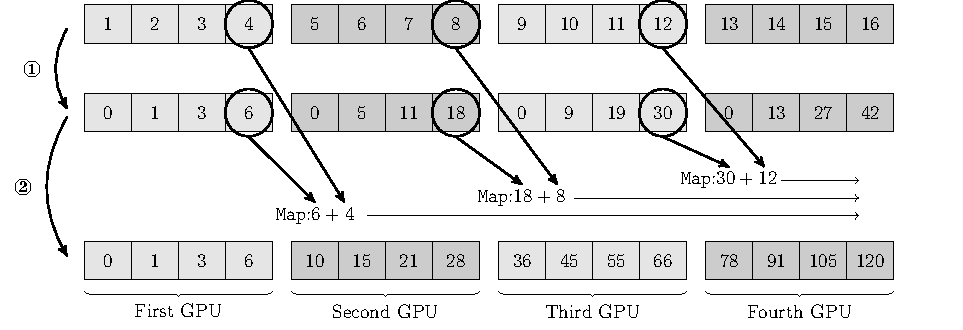
\includegraphics[width=.9\textwidth]{ASHES/scan}
    \caption[Implementation of the \scan skeleton.]%
            {Implementation of the \scan skeleton visualized for four \GPUs:
            (1) All \GPUs scan their parts independently.
            (2) \map skeletons are created automatically and
             executed to produce the result.}
    \label{fig:scan:impl}
\end{figure*}

%The \SkelCL implementation of the \scan skeleton assumes the \GPUs to have a fixed order, such that each \GPU (except the first one) has a predecessor:
%\begin{enumerate}
% \item Every \GPU executes a local scan algorithm for its local part of data;
% \item The results of all \GPUs are downloaded to the \CPU;
% \item For each \GPU (except the first one), a \map skeleton is implicitly created that combines the result of the \GPU's predecessors with all elements of its part using the user-defined operation of the \scan skeleton;
% \item The newly created \map skeletons compute the final results on all \GPUs.
%\end{enumerate}
The output vector is block-distributed among all \GPUs.





\subsubsection{The Stencil Skeleton}
\label{sec:skelcl:stencil}
In stencil applications, the same computation is performed for each element of a container where the computation depends upon neighboring values.
In \autoref{section:skelcl-programming-model} we defined the \stencil skeleton to simplify the development of stencil applications.
The \SkelCL library provides two implementations of the \stencil skeleton.
The first one, called \code{MapOverlap}, supports simple stencil computations;
the second one, called \code{Stencil}, provides support for more complex stencil computations possibly executed iteratively.
In order to achieve high performance, both implementations \code{MapOverlap} and \code{Stencil} use the \GPU's fast local memory.
Both implementations perform the same basic steps on the \GPU:
first, the data is loaded from the global memory into the local memory;
then, the customizing function is called for every data element by passing a pointer to the element's location in the local memory;
finally, the result of the customizing function is copied back into the global memory.
Although both implementations perform the same basic steps, different strategies are implemented for loading the data from the global into the local memory.

In this subsection, we will start by discussing the \code{MapOverlap} implementation and then discuss the \code{Stencil} implementation.
Finally, we will discuss the implementation of the \stencil skeleton for multi-device systems.

\paragraph{The MapOverlap implementation}

We will use the Gaussian blur as an example application to discuss the \code{MapOverlap} implementation.
The Gaussian blur is a standard image processing algorithm used, among other things, for noise reduction.
The color of every pixel of an image is modified by computing a weighted average of the neighboring pixel color values.
The application will be discussed in more detail in \autoref{sec:gauss}.

\autoref{lst:mapoverlap} shows how the \code{MapOverlap} skeleton implementation is used to express the Gaussian blur.
The \code{mapOverlap} function in \autoref{lst:mapoverlap:factory} is customized with a lambda expression which uses its argument, a \code{Neighborhood} object (\autoref{lst:mapoverlap:neighborhood}), to access the neighboring elements with relative indices (\autoref{lst:mapoverlap:indices1} and \autoref{lst:mapoverlap:indices2}).
The second and third argument of the factory function define the range of the stencil shape and the border handling method (\autoref{lst:mapoverlap:borderHandling}).
The actual computation of the Gaussian blur is omitted from \autoref{lst:mapoverlap} for brevity reasons.

\begin{lstlisting}[%
caption={[Implementation of Gaussian blur using the \stencil skeleton.]%
         Implementation of Gaussian blur using the \code{MapOverlap} implementaion of the \stencil skeleton.},%
float={tb},
label={lst:mapoverlap}]
auto gauss = mapOverlap($\label{lst:mapoverlap:factory}$
  [](Neighborhood<char>& in_img) {$\label{lst:mapoverlap:neighborhood}$
      char ul = in_img[{-1, -1}];$\label{lst:mapoverlap:indices1}$
      ...
      char lr = in_img[{+1, +1}];$\label{lst:mapoverlap:indices2}$
      return computeGaussianBlur(ul, ..., lr); },
  1, BorderHandling::NEUTRAL(0));$\label{lst:mapoverlap:borderHandling}$
\end{lstlisting}


\begin{lstlisting}[%
caption={\OpenCL kernel created by the \code{MapOverlap} implementation for the Gaussian blur application.},%
float={tb},
label={lst:mapoverlap:impl}]
#define RANGE (1)   #define NEUTRAL (0)
struct {$\label{lst:mapoverlap:impl:struct:start}$
  local char* data; int row; int col; } char_neighborhood_t;$\label{lst:mapoverlap:impl:struct:end}$

char get(char_neighborhood_t* m, int x, int y) {$\label{lst:mapoverlap:impl:get:start}$
  return m->data[/*computed from RANGE, row, col, x, y*/]; }$\label{lst:mapoverlap:impl:get:end}$

char USER_FUNC(char_neighborhood_t* in_img) {
  char ul = get(in_img, -1, -1);
  ...
  char lr = get(in_img, +1, +1);
  return computeGaussianBlur(ul, ..., lr); }

kernel void mapoverlap(global char* in, global char* out,$\label{lst:mapoverlap:impl:kernel:start}$
          local char* buffer, int numCols, int numRows) {
  ... // load part of in into local buffer$\label{lst:mapoverlap:impl:copy}$
  char_neighborhood_t M;   M.data = buffer;
  M.row = get_local_id(1); M.col = get_local_id(0);
  barrier(CLK_LOCAL_MEM_FENCE);$\label{lst:mapoverlap:impl:barrier}$
  if (/* not out of bound */)
    out[index] = USER_FUNC(&M); }$\label{lst:mapoverlap:impl:call}$
\end{lstlisting}

\autoref{lst:mapoverlap:impl} shows a sketch of the \OpenCL kernel created by the \code{MapOverlap} implementation.
To represent the \code{Neighborhood} object in \OpenCL, a C \code{struct} is created (\autoref{lst:mapoverlap:impl:struct:start}---\autoref{lst:mapoverlap:impl:struct:end}).
A helper function \code{get} (\autoref{lst:mapoverlap:impl:get:start}---\autoref{lst:mapoverlap:impl:get:end}) is created which handles the read access to the data hold by the neighborhood object.
The kernel function \code{mapoverlap}, defined in \autoref{lst:mapoverlap:impl:kernel:start}, first loads the data required by a work-group into a local buffer stored in the fast local \GPU memory (\autoref{lst:mapoverlap:impl:copy}).
It then prepares a neighborhood object and passes it to the customizing function after a boundary check was performed.
A barrier (\autoref{lst:mapoverlap:impl:barrier}) ensures that the loading into the fast local memory has been completed before any work-item executes the customizing function.

Loading of the data into the fast local memory is lengthy and involves performing the boundary checks, therefore, it is not shown in \autoref{lst:mapoverlap:impl}.
%
\begin{figure}
  \begin{centering}
    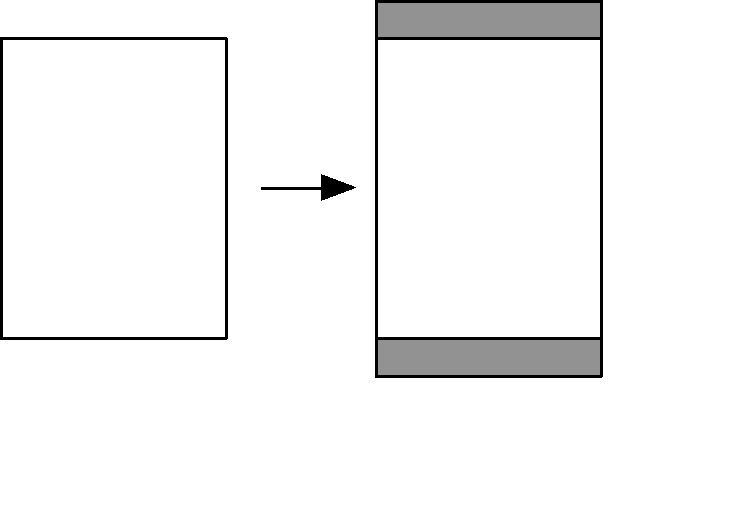
\includegraphics[width=.29\textwidth]{HiStencils/map_overlap}
    \caption[The \code{MapOverlap} implementation of the \stencil skeleton]{The \code{MapOverlap} implementation of the \stencil skeleton prepares a matrix by copying data on the top and bottom}
    \label{fig:mapoverlap:preparation}
    \vspace{-.5em}
  \end{centering}
\end{figure}
%
To minimize the overhead on the \GPU, the \code{MapOverlap} implementation prepares the input matrix on the \CPU before uploading it to the \GPU:
padding elements are appended; they are used to avoid out-of-bounds memory accesses to the top and bottom of the input matrix, as shown in \autoref{fig:mapoverlap:preparation}.
This slightly enlarges the input matrix, but it reduces branching on the \GPU due to avoiding some out-of-bound checks.
In \SkelCL a matrix is stored row-wise in memory on the \CPU and \GPU, therefore, it would be complex and costly to add padding elements on the left and right of the matrix.
To avoid out-of-bound accesses for these regions, the boundary checks are performed on the \GPU.

\paragraph{The Stencil implementation}

We use an iterative stencil application simulating heat flow to discuss the \code{Stencil} implementation.
The application simulates heat spreading from one location and flowing throughout a two-dimensional simulation space.
Let us assume that the heat flows from left to right as indicated by the arrows in \autoref{fig:stencil:first:shape}.
The heat value of a cell is updated based on its (left) neighboring cells.
Multiple iteration steps are required to simulate the flow of heat over a longer distance.

\begin{figure}[t]
  \begin{minipage}[b]{.38\textwidth}
    \centering
    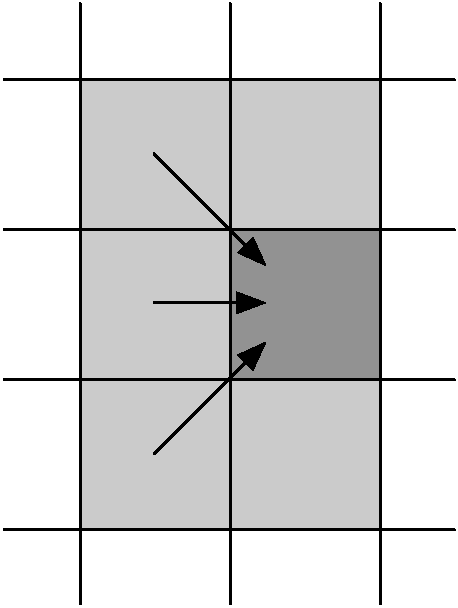
\includegraphics[width=.65\textwidth]{Figures/HiStencils/heat_transfer}
    \caption{Stencil shape for heat simulation}
    \label{fig:stencil:first:shape}
  \end{minipage}
  \hfill %\hspace{.05\textwidth}
  \begin{minipage}[b]{.55\textwidth}
    \begin{lstlisting}[%
      caption={[Heat simulation with the \stencil skeleton]Heat simulation with the \stencil skeleton\vspace{-.9em}},%
      label={lst:stencil:first}]
auto heatSim = skelcl::stencil(
 [](Neighborhood<char>& in) {$\label{lst:stencil:first:func:start}$
  char lt = in[{-1, -1}];
  char lm = in[{-1,  0}];
  char lb = in[{-1, +1}];
  return computeHeat(lt,lm,lb);},$\label{lst:stencil:first:func:end}$
 StencilShape(1, 0, 1, 1),$\label{lst:stencil:first:shape}$
 BorderHandling::NEUTRAL(255));$\label{lst:stencil:first:border}$
heatSim(100_iterations,$\label{lst:stencil:first:iterations}$
        simulationSpace);
    \end{lstlisting}
  \end{minipage}%
\end{figure}

\autoref{lst:stencil:first} shows the implementation of an iterative stencil application simulating heat transfer in \SkelCL.
The application developer specifies the customizing function (\autoref{lst:stencil:first:func:start}---\autoref{lst:stencil:first:func:end}), as well as the extents of the stencil shape (\autoref{lst:stencil:first:shape}) and the out-of-bound handling (\autoref{lst:stencil:first:border}).
The \code{Stencil} implementation allows the stencil shape's extents to be specified using four values for each of the directions:
up, right, down, and left.
In the example in \autoref{lst:stencil:first}, the heat flows from left to right, therefore, no accesses to the elements to the right are necessary and the stencil space's extents are specified accordingly (note the $0$ in \autoref{lst:stencil:first:shape} representing the extent to the right).
\autoref{fig:stencil:first:shape} illustrates this situation: the dark gray element is updated by using the values from the left.
The specified stencil shape's extent is highlighted in light gray.
In our current implementation, the user has to explicitly specify the stencil shape's extents, which is necessary for performing the out-of-bound handling on the \GPU.
In future work, the stencil shape could be inferred from the customizing function using source code analysis in many common cases.
This would help to avoid inconsistencies and free the user from specifying this information explicitly.

Stencil applications often perform stencil computations iteratively, like the heat transfer example which performs multiple iteration steps in order to simulate the transfer of heat over time.
The \code{Stencil} implementation supports iterative execution, which is especially challenging to implement on multi-device systems as we will see later.
On execution of the skeleton, the number of iterations to be performed is specified by the user as the first argument (\autoref{lst:stencil:first:iterations}).
This could be extended in the future, so that the user specifies a function to check if a application specific condition is met and stop the iteration.

The \OpenCL kernel created by the \code{Stencil} implementation looks similar to the \code{MapOverlap} implementation presented in \autoref{lst:mapoverlap:impl}.
The \code{Stencil} implementation uses a slightly different strategy than the \code{MapOverlap} implementation in order to enable the usage of different out-of-bound modes and stencil shapes when using several \stencil skeletons in a sequence, which we discuss in the next paragraph.
To understand why the strategy used by the \code{MapOverlap} implementation is not sufficient for stencil sequences let us consider a situation where two stencil computations are performed one after another and the two stencil shapes used are different.
This cannot be implemented efficiently using \code{MapOverlap}'s implementation strategy, as the input matrix is extended on the \CPU as specified by the first stencil shape.
Therefore, data would have to be downloaded to the \CPU between executions and the data layout would have to be changed.
To avoid this problem, the \code{Stencil} implementation does not append padding elements on the \CPU, but rather manages all out-of-bounds accesses on the \GPU, which slightly increases branching in the code, but enables a more flexible usage of the skeleton.


\paragraph{Sequence of Stencil Operations}
Many real-world applications perform different stencil operations in sequence, like the popular \emph{Canny algorithm}~\cite{NixonAg2012} used for detecting edges in images.
For the sake of simplicity, we consider a version which applies the following steps:
1)~a noise reduction operation is applied, e.\,g., a Gaussian blur;
2)~an edge detection operator like the Sobel filter is applied;
3)~the so-called non-maximum suppression is performed, where all pixels in the image are colored black except pixels being a local maximum;
4)~a threshold operation is applied to produce the final result.
A more complex version of the algorithm performs the edge tracking by hysteresis as an additional step.

Using the \SkelCL library, each single step of the Canny algorithm can be expressed using the \stencil skeleton, as shown in \autoref{lst:stencil:canny}.
The threshold operation performed as the last step, does not need access to, neighboring elements, because the user function only checks the value of a single pixel.
The \code{Stencil} implementation automatically uses the implementation of the simpler (and thus faster) \map skeleton when the user specifies a stencil shape whose extents are $0$ in all directions.
The single steps are combined into a single object of type \code{StencilSequence} which can be executed like a \stencil skeleton.
On execution, it passes its input data to the first stencil defined in the sequence, which passes its output to the next stencil, and so forth.

\begin{lstlisting}[%
  caption={Structure of the Canny algorithm implemented by a sequence of skeletons.},%
  float={tb},
  label={lst:stencil:canny}]
auto gauss     = stencil(...);
auto sobel     = stencil(...);
auto nms       = stencil(...);
auto threshold = stencil(...);

StencilSequence<Pixel(Pixel)>
    canny(gauss, sobel, nms, threshold);
\end{lstlisting}

\paragraph{Targeting Multi-\GPU Systems}
The implicit and automatic support of systems with multiple \OpenCL devices is one of the key features of \SkelCL.
By using distributions, \SkelCL completely liberates the user from error-prone and low-level explicit programming of data (re)distributions on multiple \GPUs.

The \code{MapOverlap} implementation uses the overlap distribution with \textit{border regions} in which the elements calculated by a neighboring device are located.
When it comes to iteratively executing a skeleton, data has to be transferred among devices between iteration steps, in order to ensure that data for the next iteration step is up-to-date.
As the \code{MapOverlap} implementation does not explicitly supports iterations, its implementation is not able to exchange data between devices besides a full down- and upload of the matrix.
% In addition, data exchange has to be performed after each iteration.

The \code{Stencil} implementation explicitly supports iterative execution and, therefore, only exchanges elements from the border region and does not perform a full down- and upload of the matrix, as the \code{MapOverlap} implementation does.
\autoref{fig:syncDevices} shows the \textit{device synchronizations}, \ie, the data exchange performed between two iterations by the \code{Stencil} implementation.
Only the appropriate elements in the \emph{inner border region}, \ie, the border regions adjacent to two \OpenCL devices, are downloaded and stored as \texttt{std::vector}s in a \texttt{std::vector}.
Within the outer vector, the inner vectors are swapped pair-wise on the host, so that the inner border regions can be uploaded in order to replace the out-of-date border regions.

\begin{figure}[tb]
  \centering
  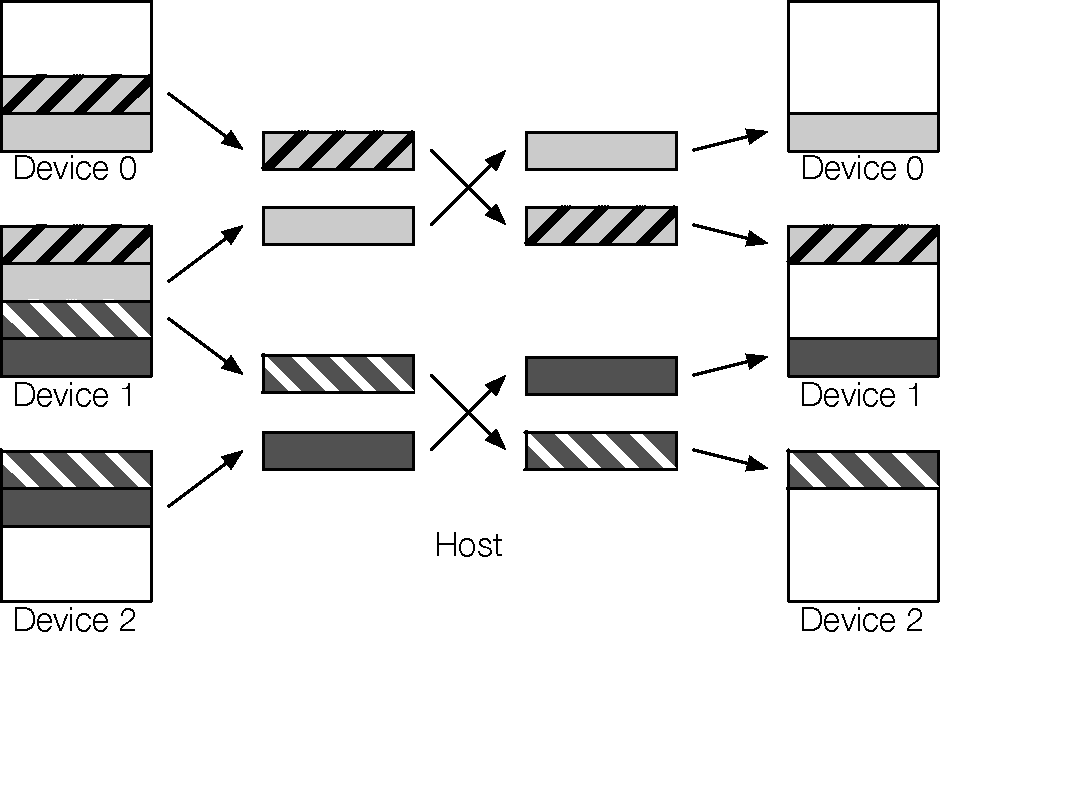
\includegraphics[width=.75\columnwidth]{HiStencils/data_exchange}
  \caption[Device synchronization for three devices during the execution of the \stencil skeleton.]
          {\small Device synchronization for three devices. Equally patterned and colored chunks represent the border regions and their matching inner border region. After the download of the appropriate inner border regions, they are swapped pair-wise on the host. Then the inner border regions are uploaded in order to replace the outdated border regions.}
  \label{fig:syncDevices}
  \vspace{1em}
\end{figure}


By enlarging the number of elements in the border regions, multiple iteration steps can be performed on each device before exchanging data.
However, this introduces redundant computations, such that a trade-off between data exchange and redundant computations has to be found.
For the \code{Stencil} implementation, the user can specify the number of iterations between device synchronizations.
In \cite{Breuer2014} the effects of exploring this parameter space is discussed.
For the investigated applications, the effect of choosing different numbers of iterations between device synchronization was not very large.


\subsubsection{The \allpairs Skeleton}
The \allpairs skeleton defined in \autoref{section:skelcl-programming-model} applies a customizing function to all pairs of vectors from two matrices.
There exist two version of the skeleton: the generic \allpairs skeleton introduced in \autoref{sec:allpairs_skeleton} and the specialized \allpairs skeleton introduced in \autoref{sec:opt_allpairs_skeleton}.
In the specialized version the customizing function is expressed as a composition of the \zip and \reduce skeleton.

In this subsection, we will first discuss the generic and then the specialized implementation.
We will also estimate the performance benefit gained by the specialized implementation.
Finally, we will discuss the implementation of the \allpairs skeleton on multi-device systems.

\paragraph{The Generic Allpairs Skeleton}
\begin{lstlisting}[%
caption={Matrix multiplication expressed using the generic \allpairs skeleton.},%
float=t,%
numbers=left,%
label={lst:allpairs:generic:impl}]
auto mm = allpairs([](const Vector<float>& a,
                      const Vector<float>& b) {
                        float c = 0.0f;
                        for (int i = 0; i < a.size(); ++i)
                          c += a[i] * b[i];
                        return c; });
\end{lstlisting}

\autoref{lst:allpairs:generic:impl} shows the program for computing matrix multiplication using the generic \allpairs skeleton.
The implementation of the customizing function is straightforward.
It is expressed as a lambda expression that receives a pair of vectors, multiplies their elements and sums them up.

\autoref{lst:allpairs:generic:kernel} shows the \OpenCL kernel created after adding and adapting the generic allpairs implementation.
The customizing function (\autoref{lst:allpairs:generic:kernel:funcStart}---\autoref{lst:allpairs:generic:kernel:funcEnd}) has been transformed by the \code{skelclc} compiler.
The vector class has been replaced by an \OpenCL representation (defined in \autoref{lst:allpairs:generic:kernel:structStart} and \autoref{lst:allpairs:generic:kernel:structEnd}) and the element access to the vectors has been replaced by computations of the matching indices.
This implementation assumes that the rows of the first matrix are combined with the columns of the second matrix, as it is required for the matrix multiplication.
% The implementation could easily be extended to support different behavior as well.

The \code{allpairs} kernel function prepares instances of the \code{struct} replacing the vector class in \autoref{lst:allpairs:generic:kernel:prepareStart} and \autoref{lst:allpairs:generic:kernel:prepareEnd}.
After performing a boundary check, the customizing function is called in \autoref{lst:allpairs:generic:kernel:call}.
This \OpenCL kernel is executed once for every element of the output matrix $C$.

\begin{lstlisting}[%
caption={\OpenCL kernel used in the implementation of the generic \allpairs skeleton.},%
float=t,%
numbers=left,%
label={lst:allpairs:generic:kernel}]
struct {$\label{lst:allpairs:generic:kernel:structStart}$
  global float* data; int size; int index; } float_matrix_t;$\label{lst:allpairs:generic:kernel:structEnd}$

float USER_FUNC(float_matrix_t* a, float_matrix_t* b) {$\label{lst:allpairs:generic:kernel:funcStart}$
   float c = 0.0f;
   for (int i = 0; i < a->size; ++i) {
     c +=   a->data[a->index * a->size + i]
          * b->data[i * b->size + b->index]; }
   return c; }$\label{lst:allpairs:generic:kernel:funcEnd}$

kernel void allpairs(const global float* Ap,
                     const global float* Bp,
                           global float* Cp,
                     int n, int d, int m) {
  int col = get_global_id(0); int row = get_global_id(1);
  float_matrix_t A; A.data = Ap; Am.size = d; A.index = row;$\label{lst:allpairs:generic:kernel:prepareStart}$
  float_matrix_t B; B.data = Bp; Bm.size = m; B.index = col;$\label{lst:allpairs:generic:kernel:prepareEnd}$
  if (row < n && col < m)
    Cp[row * m + col] = USER_FUNC(&A, &B); }$\label{lst:allpairs:generic:kernel:call}$
\end{lstlisting}

This generic implementation makes no assumption about the order in which the customizing function (\texttt{USER\_FUNC}) accesses the elements of its two input vectors.
In this generic case, we cannot assume that the two vectors fit entirely into the fast but restricted \GPU local memory.
Therefore, we have to use only the slower global memory in the generic implementation.
On modern \GPUs, accesses to the global memory are very expensive, taking up to 800 processor cycles, as compared to only few cycles required to access the local memory~\cite{CUDAProgrammingGuide}.

Let us assume targeting \GPU architectures and estimate the number of global (and, therefore, expensive) memory accesses required for computing an element of the matrix multiplication in the generic case.
One global memory read access for every element of both input vectors is performed, and a single global memory write access is required to write the result into the output matrix.
Therefore,
\begin{equation}
  n\cdot m\cdot (d + d + 1)
  \label{eq:mm:accesses}
\end{equation}
global memory accesses are performed in total, where $n$ and $m$ are the height and width of matrix $C$ and $d$ is the width of $A$ and the height of $B$.
By using the fast but small local memory, this number of global memory accesses can be reduced and, thus, performance can be improved, as we will see in the next paragraph.
Using the local memory for matrix multiplication is a well-known optimization which we systematically apply to a generic skeleton, rather than to a particular application as usually done in the literature.

\paragraph{The Specialized Allpairs Skeleton}
\autoref{lst:allpairs:special:impl} shows matrix multiplication expressed using the specialized \allpairs skeleton.
\begin{lstlisting}[%
caption={Matrix multiplication expressed using the specialized \allpairs skeleton.},%
float=t,%
numbers=left,%
label={lst:allpairs:special:impl}]
auto mult  = zip([](float x, float y){return x*y;});
auto sumUp = reduce([](float x, float y){return x+y;}, 0);
auto mm    = allpairs(sumUp, mult);
\end{lstlisting}
%
By expressing the customizing function of the \allpairs skeleton as a \zip-\reduce composition, we provide to the skeleton implementation additional semantic information about the memory access pattern of the customizing function, thus allowing for improving the performance.
Our idea of optimization is based on the \OpenCL programming model that organizes \emph{work-items} in \emph{work-groups} which share the same \GPU local memory.
By loading data needed by multiple work-items of the same work-group into the local memory, we can avoid repetitive accesses to the global memory.

\begin{figure}[b]
  \centering
  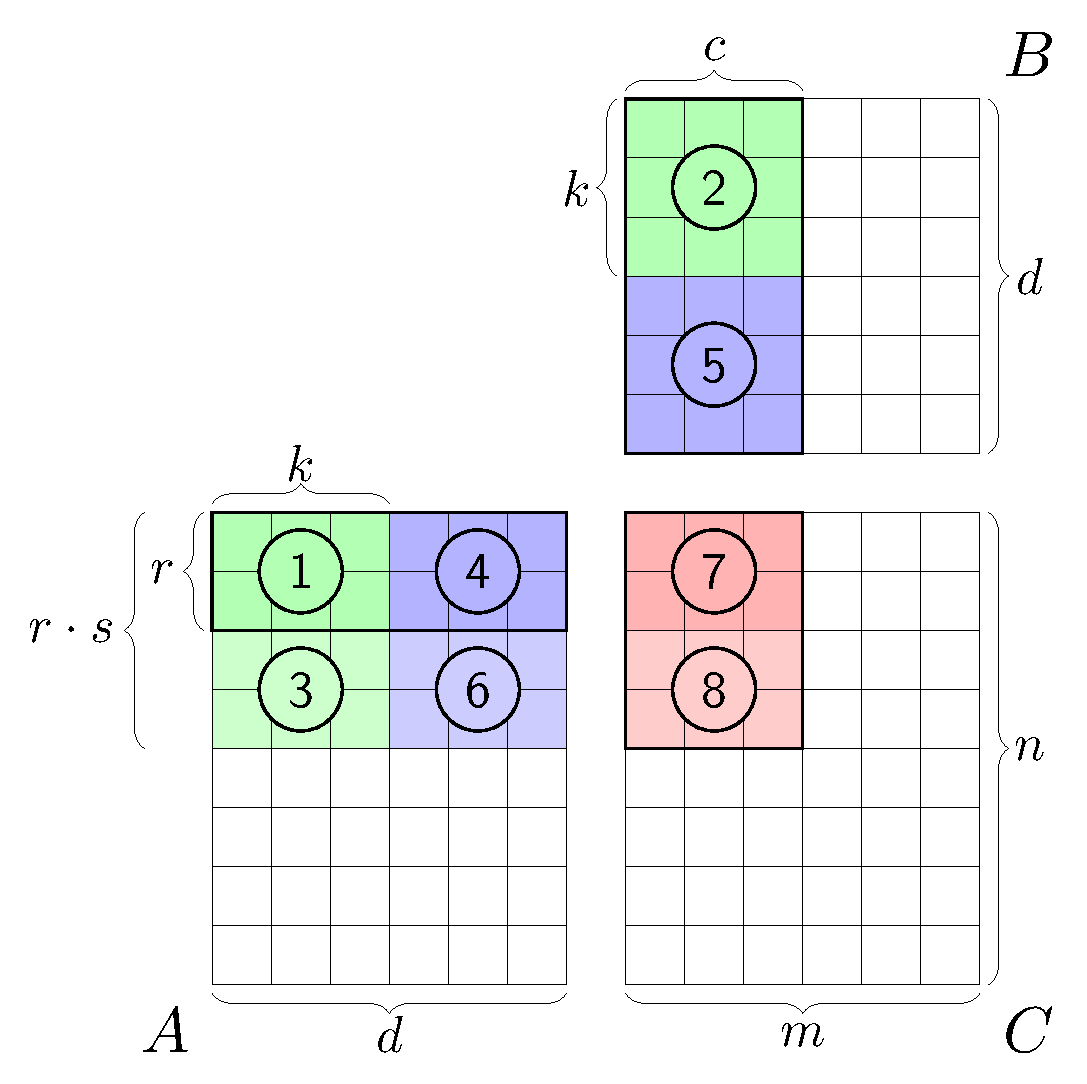
\includegraphics[width=.4\textwidth]{HLPP/memory_access}
  \caption{Implementation schema of the specialized \allpairs skeleton.}
  \label{fig:memory_access}
\end{figure}
For the \allpairs skeleton with the \zip-\reduce customizing function, we can adopt the implementation schema for \GPUs from~\cite{SarjeAl2013}, as shown in \autoref{fig:memory_access}.
We allocate two arrays in the local memory, one of size $r\times k$ ($r=2$, $k=3$ in \autoref{fig:memory_access}) for elements of $A$ and one of size $k\times c$ ($c=3$ in \autoref{fig:memory_access}) for elements of $B$.
A work-group consisting of $c\times r$ work-items computes $s$ blocks ($s=2$ in \autoref{fig:memory_access}) of the result matrix $C$.
In \autoref{fig:memory_access}, the two blocks marked as \circled{7} and \circled{8} are computed by the same work-group as follows.
In the first iteration, the elements of blocks \circled{1} and \circled{2} are loaded into the local memory and combined following the \zip-\reduce pattern.
The obtained intermediate result is stored in block \circled{7}.
Then, the elements of block \circled{3} are loaded and combined with the elements from \circled{2} which still reside in the local memory.
The intermediate result is stored in block \circled{8}.
In the second iteration, the algorithm continues in the same manner with blocks \circled{4}, \circled{5}, and \circled{6}, but this time, the elements of the blocks are also combined with the intermediate results of the first iteration, which are stored in blocks \circled{7} and \circled{8}.
The advantage of computing multiple blocks by the same work-group is that we keep the elements of $B$ in the local memory when computing the intermediate results, \ie, we do not reload block \circled{2} twice for the computation of blocks \circled{7} and \circled{8}.

Every element loaded from the global memory is used by multiple work-items:
\eg, the upper left element of block \circled{1} is loaded only once from the global memory, but used three times:
in the computation of the upper left, upper middle, and upper right elements of \circled{7}.
In general, every element loaded from $A$ is reused $c$ times, and every element from $B$ is reused $r\cdot s$ times.
As the intermediate results are stored in the global memory of matrix $C$, we perform two additional memory accesses (read/write) for every iteration, \ie, $2\cdot \frac{d}{k}$ in total.
Therefore, instead of $n\cdot m\cdot (d + d + 1)$ (see \autoref{eq:mm:accesses}) global memory accesses necessary when using the non-specialized skeleton only
\begin{equation}
  n\cdot m\cdot (\frac{d}{r\cdot s} + \frac{d}{c} + 2\cdot \frac{d}{k})
\end{equation}
global memory accesses are performed.
By increasing the parameters $s$ and $k$, or the number of work-items in a work-group ($c$ and $r$), more global memory accesses can be saved.
However, the work-group size is limited by the \GPU hardware.
While the parameters can be chosen independently of the matrix sizes, we have to consider the amount of available local memory.
\cite{Friese2013}~and~\cite{SarjeAl2013}~discuss how suitable parameters can be found by performing runtime experiments.
In~\cite{Friese2013} the parameters $c = 32$, $r=8$, $s=32$, and $k=64$ are used on modern \GPU hardware showing good performance.

We will report measurements of the performance difference for the two skeleton implementations on real hardware in \autoref{chapter:skelcl-evaluation}.

\paragraph{The Allpairs Skeleton using Multiple GPUs}
\label{sec:allpairs:multi_gpu}
\begin{figure}[b]
  \centering
  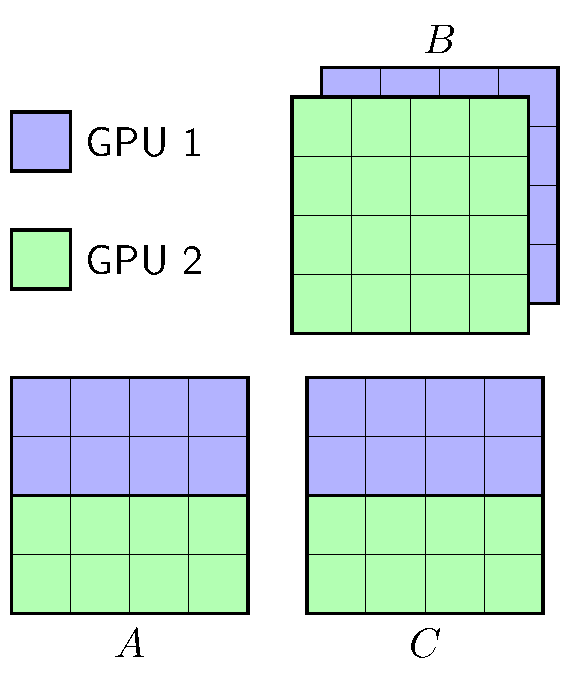
\includegraphics[width=.3\textwidth]{HLPP/multi_gpu}
  \caption[Data distributions used for the \allpairs skeleton for a system with two \GPUs.]%
          {Data distributions used for a system with two \GPUs: matrices $A$ and $C$ are \emph{block} distributed, matrix $B$ is \emph{copy} distributed.}
  \label{fig:multi_gpu}
\end{figure}

The \allpairs skeleton can be efficiently implemented not only on systems with a single \GPU, but on multi-\GPU systems as well.
The necessary data distribution can be easily expressed using two of \SkelCL's \emph{distributions}, as shown in \autoref{fig:multi_gpu}:
Matrix $B$ is \emph{copy} distributed, \ie, it is copied entirely to all \GPUs in the system.
Matrix $A$ and $C$ are \emph{block} distributed, \ie, they are row-divided into as many equally-sized blocks as \GPUs are available;
each block is copied to its corresponding \GPU.
Following these distributions, each \GPU computes one block of the result matrix $C$.
In the example with two \GPUs shown in \autoref{fig:multi_gpu}, the first two rows of $C$ are computed by \GPU 1 and the last two rows by \GPU 2.
The \allpairs skeleton automatically selects these distributions, therefore, the same source code can be used when using a single \GPU or multiple \GPUs.











\subsection{Memory Management Implementation}
\label{section:skelcl-library:memory-management}
In the \SkelCL programming model, the user manages memory using \emph{container data types}.
In the \SkelCL library, the two container data types -- vector and matrix -- are implemented as template classes.
This generic implementation allows for storing data items of any primitive C/\Cpp data type (\eg, \code{int}), as well as user-defined data structures (\code{struct}s).
The implementations follow the \emph{resource acquisition is initialization} (RAII) idiom, which means that they automatically allocate needed resources and free them automatically when the lifetime of the container ends.

\paragraph{The SkelCL Vector}
The \SkelCL vector replicates the interface of the vector from the \Cpp Standard Template Library (\STL), \ie, it can be used as a drop-in replacement of the standard vector.
Internally, a vector comprises pointers to the corresponding areas of main memory (accessible by the host) and device memory.
The vector holds one pointer for the host and one pointer for each device available.
Memory on the devices is allocated automatically, according to the distribution of the vector:
while for a single distributed vector only memory on a single device is allocated, for a vector distributed with the copy, block, or overlap distribution memory on all devices is allocated.
The selected distribution obviously also influences how big the buffers allocated on the devices will be.

Before the execution of a skeleton, the input vector's implementation ensures that all of its data is available on the devices.
This might result in implicit data transfers from the host memory to device memory.
The data of the output vector is not copied back to the host memory but rather resides in the device memory.
Before every data transfer, the vector implementation checks whether the data transfer is necessary;
only then the data is actually transferred.
Hence, if an output vector is used as the input to another skeleton, no further data transfer is performed.
This \emph{lazy copying} in \SkelCL defers data transfers as long as possible or avoids them completely and, thus, minimizes the costly data transfers between host and device.
While all data transfers are performed implicitly by \SkelCL, we understand that experienced application developers may want to have a fine-grained control over the data transfers between host and devices.
For that purpose, \SkelCL offers a set of \APIs which developers can use to explicitly initiate and control the data transfer to and from the devices.

% Implementing such data transfers in \OpenCL manually is a cumbersome task:
% data has to be downloaded to the host before it can be uploaded to other devices, including the corresponding length and offset calculations;
% this results in a lot of low-level code which is completely hidden when using \SkelCL.


\paragraph{The SkelCL Matrix}
The \SkelCL matrix offers an easy to use interface similar to the interface of the vector.
Data is stored in the row-major order and iterators are provided to iterate first over rows and then inside of a single row to access a particular element.
For the copy, block, and overlap distributions, the matrix is divided across rows.
A single row is never split across multiple devices, which simplifies the memory management.
Besides offering an interface to access elements on the host, the matrix also offers an interface for accessing elements on the device by using two-dimensional indices.
This frees the application developer from performing cumbersome index calculations manually.










\subsection{Data Distribution Implementation}
\label{section:skelcl-library:distribution}
The data distributions determine how the data of a container is distributed across multiple devices.
In the \SkelCL library implementation, there exists a class for each data distribution encapsulating the behavior of the distribution.
Every container stores its current data distribution as a member variable.
When the data of the container has to be transferred to or from the devices, the data distribution object is invoked to perform the data transfer operation.

% The data distribution of a container can be changed at runtime either explicitly by the programmer or implicitly by the \SkelCL implementation.
% A change of distribution implies data exchanges between multiple devices and the host, which are performed implicitly by \SkelCL.
% These implicit data exchanges are also performed lazily, \ie, only if really necessary, as described in the previous subsection.

% A special situation arises when the distribution is changed from the \emph{copy} distribution, where each device holds its own full copy of the data.
% In such a case, each device may hold a different version of the container as data modifications are only performed locally on the device.
% In order to maintain \SkelCL's concept of a self-contained container, these different versions must be combined using a user-specified function when the distribution is changed.
% If no function is specified, the copy of the first device is taken as the new version of the container; the copies of the other devices are discarded.



